% Chapter Ethem

\chapter{Electro-Thermal Modelization of the RED Dectectors}

\label{ChapterEthem} % Change X to a consecutive number; for referencing this chapter elsewhere, use \ref{ChapterX}

%----------------------------------------------------------------------------------------
%	BEGING CHAPTER
%----------------------------------------------------------------------------------------

\section{Basic Modelization of Cryogenic Bolometers}

Even though the design of the RED bolometers is quite simple, a complete modelization of its behavior requires quite some time and efforts. However, it is possible to gain some insight from a very simplified modelization (see fig \ref{bolo-model}): we consider a single thermal bath of thermal capacity $C$ and temperature $T$ thermalized by a conductance $G$ to the cryostat at temperature $T_{cryo}$. We consider the temperature of the NTD resistance $R$ to be $T$. With a constant polarization current $I$, the NTD delivers a Joule power $P_J = RI^2$ into the bolometer and the voltage $V=RI$ is amplified by the FET-based electronic. It should be noted that the constant current $I$ is obtained by passing a triangular voltage wave through an electric capacity (this presents some advantages, more will be discuss).

\begin{figure}
\centering
\captionsetup{justification=centering}
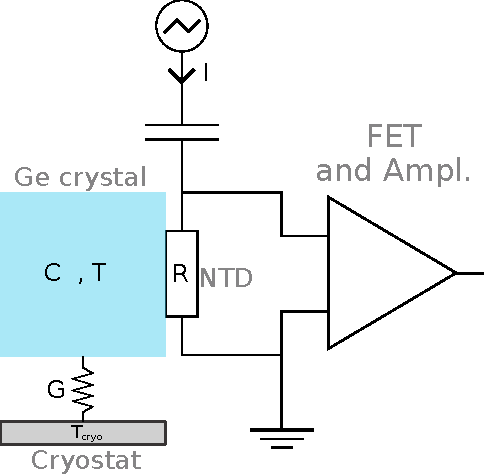
\includegraphics[width=0.3\textwidth]{graphics/bolo_simple.pdf}
\caption{\label{bolo-model} \em Simplified scheme of a RED bolometer coupling a thermal system (left side) and an electrical system (right side). }
\end{figure}

Here are some hints and info to help you understand the behavior of the bolometers (calculation and discussion in parallel with the measurements):
\begin{itemize}
	\item The heat power injected by the cryostat into the bolometer is $$P_{cryo} = G \left( T_{cryo} - T\right) \quad [\textrm{in } Watt]$$ In the considered simplified system, only the limiting conductance is considered (the lowest) which is generally the electron-phonon coupling (more in discussion..)
	\item A lot can be understand from studying the stationary state ($dT/dt=0$) and the time resolution (useful to introduce $\Delta T = T - T_{eq}$) of the heat equilibrium equation in the stationary state. Just recall that with $t$ the time and $U$ the energy of the thermal bath $$\frac{dU}{dt} = C \frac{dT}{dt} \quad [\textrm{in }  Joule]$$
	\item Some reference value for RED bolometers:
	$$ R = \mathcal{O}(1 \ G\Omega),\
	C \approx 3 \times 10^{-10} \ J.K^{-1},\
	G \approx 2 \times 10^{-8} \ W.K^{-1},\
	I = \mathcal{O}(1 \ nA),\
	T_{cryo} \approx 20 \ mK $$
	\item An optimized bolometer has the highest sensitivity $S_V$ in V/keV possible. Not to confuse with the sensitivity of the thermal sensor $\alpha$ which is usually introduced in this type of calculation 
	$$\alpha = \frac{1}{R} \frac{dR}{dT} $$
\end{itemize}


\subsection{Electro-thermal Modelization of the Detector}

In this part, the theoretical calculations used to build the detector model are presented. The study focused on the first-order resolution of the system of coupled differential equations using a linear algebra method : \cite{matrix}. It is then possible to simulate the behavior of a detector in the steady state, in the time regime and in the frequency regime, which gives access to the complete characterization of the detector.


\subsection{Model description}

\begin{figure}[!ht]
%\centering
%\resizebox{0.6\textwidth}{!}{%
%\shorthandoff{:!}\begin{circuitikz}[scale=1]
%	%	\draw [help lines, step=0.5cm] (0.25,0) grid (7.75,5);
	\node [below] at (4, 0.05) {$T_b$};
	\fill [pattern = north east lines] (2.5,0.05) rectangle (5.5,0.25);
	\draw [brown, line width = 5] (4,0.25) -- (4,1.75);
	\draw [thick] (2.5,0.25) -- (5.5,0.25);
	\draw [brown, line width = 5] (3.25, 2.5) -- (1.75, 2.5);
	\draw [brown, line width = 5] (4.75, 2.5) -- (6.25, 2.5);
	\node [right] at (4, 1)	{$G_{pb}$};
	\node [left] at (4, 1)	{$P_{pb}$};
	\node [below] at (2.5, 2.5)	{$G_{ap}$};
	\node [above] at (2.5, 2.5)	{$P_{ap}$};
	\node [below] at (5.5, 2.5)	{$G_{ep}$};
	\node [above] at (5.5, 2.5)	{$P_{ep}$};
	\draw [fill=yellow] (3.25, 1.75) rectangle (4.75, 3.25);
	\node at (4, 2.5) {$T_p, C_p$};
	\draw [fill=orange] (1.75, 1.75) rectangle (0.25, 3.25);
	\node at (1, 2.5) {$T_a, C_a$};
	\draw [fill=cyan] (6.25, 1.75) rectangle (7.75, 3.25);
	\node at (7, 2.5) {$T_e, C_a$};
	\node [anchor=south, inner sep=0] at (1, 3.5)
    	{\resizebox{2cm}{!}{% This file was created by matplotlib2tikz v0.6.10.
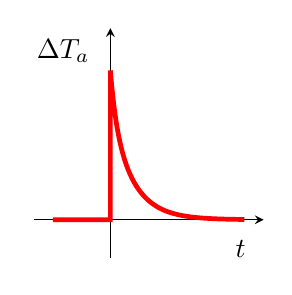
\begin{tikzpicture}

\begin{axis}[
ticks=none,
xmin=-0.2, xmax=0.4,
ymin=-0.5e-07, ymax=2.5e-07,
axis x line=center,
axis y line=center,
every axis x label/.style={at={(ticklabel cs:0.9)}, below=4pt},
every axis y label/.style={at={(ticklabel cs:0.9)}, left=4pt},
xlabel={$t$},
ylabel={$\Delta T_a$},
width=4.5cm,
height=4.5cm
]
\addplot [line width = 1.7pt, red]
table {%
-0.15 0
1e-08 0
0 1.94905773450583e-07
0.00353535353535354 1.75086151002447e-07
0.00707070707070707 1.58214334725911e-07
0.0106060606060606 1.4370498349366e-07
0.0141414141414141 1.31131841539708e-07
0.0176767676767677 1.20154073651191e-07
0.0212121212121212 1.10498558052284e-07
0.0247474747474747 1.01945886553252e-07
0.0282828282828283 9.43192935859211e-08
0.0318181818181818 8.74758993005682e-08
0.0353535353535354 8.1299781085828e-08
0.0388888888888889 7.56964899078769e-08
0.0424242424242424 7.05887084549368e-08
0.045959595959596 6.59128117256344e-08
0.0494949494949495 6.16161409749693e-08
0.053030303030303 5.76548416413408e-08
0.0565656565656566 5.39921472429897e-08
0.0601010101010101 5.05970160062528e-08
0.0636363636363636 4.74430465564955e-08
0.0671717171717172 4.45076144595586e-08
0.0707070707070707 4.17711836111647e-08
0.0742424242424242 3.92167561164711e-08
0.0777777777777778 3.68294319208594e-08
0.0813131313131313 3.45960554718693e-08
0.0848484848484848 3.25049314471608e-08
0.0883838383838384 3.05455953401098e-08
0.0919191919191919 2.8708627662862e-08
0.0954545454545454 2.69855028720667e-08
0.098989898989899 2.53684659759339e-08
0.102525252525253 2.38504312460595e-08
0.106060606060606 2.24248986152695e-08
0.10959595959596 2.10858842580303e-08
0.113131313131313 1.98278625736718e-08
0.116666666666667 1.86457173650087e-08
0.12020202020202 1.75347004576861e-08
0.123737373737374 1.64903963638234e-08
0.127272727272727 1.55086918770988e-08
0.130808080808081 1.45857497109756e-08
0.134343434343434 1.37179854696812e-08
0.137878787878788 1.29020473825878e-08
0.141414141414141 1.21347983445272e-08
0.144949494949495 1.14132998934018e-08
0.148484848484848 1.07347978270466e-08
0.152020202020202 1.00967092174591e-08
0.155555555555556 9.49661062525964e-09
0.159090909090909 8.93222735294378e-09
0.162626262626263 8.40142360402661e-09
0.166161616161616 7.9021934380375e-09
0.16969696969697 7.43265242968028e-09
0.173232323232323 6.99102995525483e-09
0.176767676767677 6.57566204137687e-09
0.18030303030303 6.18498472071477e-09
0.183838383838384 5.81752784734487e-09
0.187373737373737 5.4719093307749e-09
0.190909090909091 5.14682975298612e-09
0.194444444444444 4.84106733722839e-09
0.197979797979798 4.5534732409492e-09
0.201515151515152 4.28296714829148e-09
0.205050505050505 4.02853314017069e-09
0.208585858585859 3.78921582212947e-09
0.212121212121212 3.56411669204082e-09
0.215656565656566 3.35239073134553e-09
0.219191919191919 3.15324320491336e-09
0.222727272727273 2.96592665584594e-09
0.226262626262626 2.78973808262336e-09
0.22979797979798 2.62401628695844e-09
0.233333333333333 2.46813938158316e-09
0.236868686868687 2.32152244796522e-09
0.24040404040404 2.18361533465225e-09
0.243939393939394 2.05390058757701e-09
0.247474747474747 1.93189150423773e-09
0.251010101010101 1.81713030419968e-09
0.254545454545455 1.70918640885407e-09
0.258080808080808 1.6076548238223e-09
0.261616161616162 1.51215461781191e-09
0.265151515151515 1.42232749211878e-09
0.268686868686869 1.3378364353309e-09
0.272222222222222 1.2583644581251e-09
0.275757575757576 1.18361340336156e-09
0.279292929292929 1.11330282697358e-09
0.282828282828283 1.04716894542388e-09
0.286363636363636 9.84963645754594e-10
0.28989898989899 9.26453554498324e-10
0.293434343434343 8.71419161942022e-10
0.296969696969697 8.19653998446613e-10
0.30050505050505 7.70963859722854e-10
0.304040404040404 7.25166078149621e-10
0.307575757575758 6.82088837395062e-10
0.311111111111111 6.41570527764773e-10
0.314646464646465 6.03459139854875e-10
0.318181818181818 5.67611694232354e-10
0.321717171717172 5.33893705000791e-10
0.325252525252525 5.02178675237199e-10
0.328787878787879 4.72347622405636e-10
0.332323232323232 4.44288631966024e-10
0.335858585858586 4.17896437502591e-10
0.339393939393939 3.93072025796083e-10
0.342929292929293 3.69722265357532e-10
0.346464646464646 3.47759557029615e-10
0.35 3.27101505344391e-10
};
\end{axis}

\end{tikzpicture}}};
    \node [anchor=south, inner sep=0] at (4, 3.5)
    	{\resizebox{2cm}{!}{% This file was created by matplotlib2tikz v0.6.10.
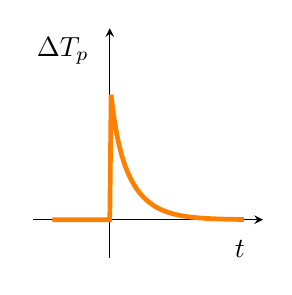
\begin{tikzpicture}

\definecolor{color0}{rgb}{1,0.647058823529412,0}


\begin{axis}[
ticks=none,
xmin=-0.2, xmax=0.4,
ymin=-0.5e-07, ymax=2.5e-07,
axis x line=center,
axis y line=center,
every axis x label/.style={at={(ticklabel cs:0.9)}, below=4pt},
every axis y label/.style={at={(ticklabel cs:0.9)}, left=4pt},
xlabel={$t$},
ylabel={$\Delta T_p$},
width=4.5cm,
height=4.5cm
]
\addplot [line width = 1.7pt, orange]
table {%
-0.15 0
1e-08 0
0 6.96368541805659e-24
0.00353535353535354 1.63176399143611e-07
0.00707070707070707 1.48010174769528e-07
0.0106060606060606 1.34895295323391e-07
0.0141414141414141 1.23468086776223e-07
0.0176767676767677 1.13437308330477e-07
0.0212121212121212 1.04569165237934e-07
0.0247474747474747 9.6675457798133e-08
0.0282828282828283 8.96042081124974e-08
0.0318181818181818 8.32322445633661e-08
0.0353535353535354 7.74593332500688e-08
0.0388888888888889 7.22035319129691e-08
0.0424242424242424 6.73975100378826e-08
0.045959595959596 6.29856326697683e-08
0.0494949494949495 5.89216479870297e-08
0.053030303030303 5.51668522742115e-08
0.0565656565656566 5.16886324595516e-08
0.0601010101010101 4.8459307338149e-08
0.0636363636363636 4.54552051530634e-08
0.0671717171717172 4.26559282807991e-08
0.0707070707070707 4.00437660952089e-08
0.0742424242424242 3.76032252420987e-08
0.0777777777777778 3.53206530016271e-08
0.0813131313131313 3.31839345070543e-08
0.0848484848484848 3.11822486108937e-08
0.0883838383838384 2.93058703676763e-08
0.0919191919191919 2.75460106137664e-08
0.0954545454545454 2.58946851090798e-08
0.098989898989899 2.43446072738405e-08
0.102525252525253 2.28890997930618e-08
0.106060606060606 2.15220213413162e-08
0.10959595959596 2.02377054550822e-08
0.113131313131313 1.90309091926043e-08
0.116666666666667 1.78967697058042e-08
0.12020202020202 1.68307672321937e-08
0.123737373737374 1.58286933182089e-08
0.127272727272727 1.48866233256637e-08
0.130808080808081 1.40008924633649e-08
0.134343434343434 1.31680747367947e-08
0.137878787878788 1.23849643284248e-08
0.141414141414141 1.16485590162039e-08
0.144949494949495 1.0956045313217e-08
0.148484848484848 1.0304785071529e-08
0.152020202020202 9.69230334102103e-09
0.155555555555556 9.11627731213953e-09
0.159090909090909 8.57452620193543e-09
0.162626262626263 8.06500196714538e-09
0.166161616161616 7.58578074763144e-09
0.16969696969697 7.13505495923382e-09
0.173232323232323 6.71112596779503e-09
0.176767676767677 6.31239728640301e-09
0.18030303030303 5.93736824626804e-09
0.183838383838384 5.58462809848333e-09
0.187373737373737 5.25285050953076e-09
0.190909090909091 4.94078841802559e-09
0.194444444444444 4.64726922404115e-09
0.197979797979798 4.37119028557055e-09
0.201515151515152 4.111514699389e-09
0.205050505050505 3.86726734587531e-09
0.208585858585859 3.63753117931072e-09
0.212121212121212 3.4214437468602e-09
0.215656565656566 3.21819392090423e-09
0.219191919191919 3.02701883066689e-09
0.222727272727273 2.84720098021137e-09
0.226262626262626 2.67806554087111e-09
0.22979797979798 2.51897780707433e-09
0.233333333333333 2.36934080531901e-09
0.236868686868687 2.2285930467763e-09
0.24040404040404 2.09620641465547e-09
0.243939393939394 1.97168417806043e-09
0.247474747474747 1.85455912461491e-09
0.251010101010101 1.74439180463596e-09
0.254545454545455 1.64076888009906e-09
0.258080808080808 1.54330157206693e-09
0.261616161616162 1.45162420065171e-09
0.265151515151515 1.36539281194944e-09
0.268686868686869 1.28428388672967e-09
0.272222222222222 1.20799312598366e-09
0.275757575757576 1.13623430873391e-09
0.279292929292929 1.06873821778733e-09
0.282828282828283 1.00525162937641e-09
0.286363636363636 9.45536362877567e-10
0.28989898989899 8.89368387025501e-10
0.293434343434343 8.36536979257968e-10
0.296969696969697 7.86843935027003e-10
0.30050505050505 7.4010282410245e-10
0.304040404040404 6.96138291071478e-10
0.307575757575758 6.54785397404927e-10
0.311111111111111 6.15889002618282e-10
0.314646464646465 5.79303182202572e-10
0.318181818181818 5.44890680139068e-10
0.321717171717172 5.12522393941935e-10
0.325252525252525 4.82076890295391e-10
0.328787878787879 4.53439949467044e-10
0.332323232323232 4.26504136787296e-10
0.335858585858586 4.01168399586413e-10
0.339393939393939 3.77337688076548e-10
0.342929292929293 3.5492259875595e-10
0.346464646464646 3.33839038997186e-10
0.35 3.14007911560752e-10
};
\end{axis}

\end{tikzpicture}}};	
    \node [anchor=south, inner sep=0] at (7, 3.5)
    	{\resizebox{2cm}{!}{% This file was created by matplotlib2tikz v0.6.10.
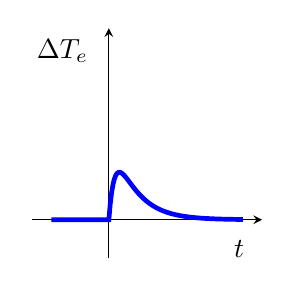
\begin{tikzpicture}

\begin{axis}[
ticks=none,
xmin=-0.2, xmax=0.4,
ymin=-0.5e-07, ymax=2.5e-07,
axis x line=center,
axis y line=center,
every axis x label/.style={at={(ticklabel cs:0.9)}, below=4pt},
every axis y label/.style={at={(ticklabel cs:0.9)}, left=4pt},
xlabel={$t$},
ylabel={$\Delta T_e$},
width=4.5cm,
height=4.5cm
]
\addplot [line width = 1.7pt, blue]
table {%
-0.15 0
1e-08 0
0 5.15986218822629e-23
0.00353535353535354 2.02319742455945e-08
0.00707070707070707 3.50283638973746e-08
0.0106060606060606 4.55829895717481e-08
0.0141414141414141 5.2854683483701e-08
0.0176767676767677 5.75967408445595e-08
0.0212121212121212 6.04003591661948e-08
0.0247474747474747 6.17289341324563e-08
0.0282828282828283 6.19451332621564e-08
0.0318181818181818 6.13322662511764e-08
0.0353535353535354 6.0111151566108e-08
0.0388888888888889 5.84534266690334e-08
0.0424242424242424 5.64920500734984e-08
0.045959595959596 5.4329586121974e-08
0.0494949494949495 5.20447391339915e-08
0.053030303030303 4.96975054505508e-08
0.0565656565656566 4.73332344043295e-08
0.0601010101010101 4.49858280406682e-08
0.0636363636363636 4.26802610766907e-08
0.0671717171717172 4.04345644105182e-08
0.0707070707070707 3.82613853431711e-08
0.0742424242424242 3.6169213865249e-08
0.0777777777777778 3.41633455563404e-08
0.0813131313131313 3.22466367949145e-08
0.0848484848484848 3.04200962489964e-08
0.0883838383838384 2.86833473567554e-08
0.0919191919191919 2.70349891927568e-08
0.0954545454545454 2.54728773405602e-08
0.098989898989899 2.39943418321705e-08
0.102525252525253 2.25963556141392e-08
0.106060606060606 2.12756641571379e-08
0.10959595959596 2.00288845812559e-08
0.113131313131313 1.88525808972803e-08
0.116666666666667 1.77433205654116e-08
0.12020202020202 1.66977164687768e-08
0.123737373737374 1.571245752772e-08
0.127272727272727 1.4784330493241e-08
0.130808080808081 1.39102349154358e-08
0.134343434343434 1.30871928548508e-08
0.137878787878788 1.23123545671688e-08
0.141414141414141 1.15830011255645e-08
0.144949494949495 1.0896544735358e-08
0.148484848484848 1.02505273303853e-08
0.152020202020202 9.64261791040749e-09
0.155555555555556 9.07060897650632e-09
0.159090909090909 8.53241234089511e-09
0.162626262626263 8.02605452431492e-09
0.166161616161616 7.54967190452406e-09
0.16969696969697 7.10150574045727e-09
0.173232323232323 6.67989716615275e-09
0.176767676767677 6.2832822247284e-09
0.18030303030303 5.91018699411838e-09
0.183838383838384 5.55922284183937e-09
0.187373737373737 5.2290818348624e-09
0.190909090909091 4.91853232202482e-09
0.194444444444444 4.62641469977975e-09
0.197979797979798 4.35163736701518e-09
0.201515151515152 4.09317287084003e-09
0.205050505050505 3.85005424236218e-09
0.208585858585859 3.62137151936202e-09
0.212121212121212 3.40626845122712e-09
0.215656565656566 3.20393938043e-09
0.219191919191919 3.01362629409614e-09
0.222727272727273 2.83461603874513e-09
0.226262626262626 2.66623769102869e-09
0.22979797979798 2.50786007718652e-09
0.233333333333333 2.35888943395577e-09
0.236868686868687 2.21876720377107e-09
0.24040404040404 2.08696795725728e-09
0.243939393939394 1.96299743622671e-09
0.247474747474747 1.84639071063342e-09
0.251010101010101 1.73671044319756e-09
0.254545454545455 1.63354525568494e-09
0.258080808080808 1.53650819110403e-09
0.261616161616162 1.44523526636046e-09
0.265151515151515 1.359384110183e-09
0.268686868686869 1.27863268140426e-09
0.272222222222222 1.20267806293949e-09
0.275757575757576 1.13123532705958e-09
0.279292929292929 1.06403646779599e-09
0.282828282828283 1.00082939654757e-09
0.286363636363636 9.41376997180387e-10
0.28989898989899 8.85456237122462e-10
0.293434343434343 8.32857331155583e-10
0.296969696969697 7.83382954796269e-10
0.30050505050505 7.36847504337837e-10
0.304040404040404 6.93076400795766e-10
0.307575757575758 6.51905435159421e-10
0.311111111111111 6.13180152505136e-10
0.314646464646465 5.76755272669063e-10
0.318181818181818 5.42494145313467e-10
0.321717171717172 5.10268237347692e-10
0.325252525252525 4.79956650785216e-10
0.328787878787879 4.51445669231489e-10
0.332323232323232 4.24628331303897e-10
0.335858585858586 3.9940402938568e-10
0.339393939393939 3.75678132210213e-10
0.342929292929293 3.53361629861074e-10
0.346464646464646 3.32370799857171e-10
0.35 3.12626893071057e-10
};
\end{axis}

\end{tikzpicture}}};
    	
%\end{circuitikz}\shorthandon{:!}
%}%
\begin{center}
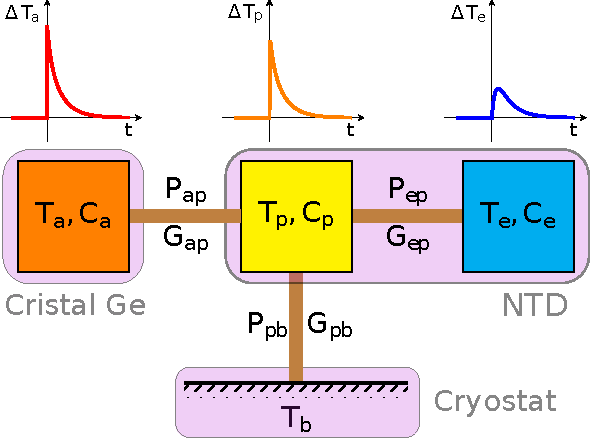
\includegraphics[width=0.6\textwidth]{Images/thermal_scheme.pdf}
\end{center}
\caption{Thermal diagram of RED1 and RED10 with representation of the diffusion of a signal created by an event in the germanium crystal. Each thermal bath is characterized by a temperature $T$ and a thermal capacity $C$. Each thermal link is associated with a thermal conductivity $G$ and a thermal power transfer $P$. The NTD sensor is modeled as a system of thermally coupled phonons (index $p$) and elecrons (index $e$). The absorber bath (index $a$) and the cryostat (index $b$) are both connected to the NTD phonon bath.}
\label{thermal-scheme}
\end{figure}

\begin{figure}[!ht]
\begin{minipage}[c]{0.45\textwidth}
\resizebox{!}{\textwidth}{%
%\shorthandoff{:!}
\begin{circuitikz}[scale=1]
	  	\draw
	 (0.5,6) node [ground, rotate=-90] {} 
	 to [european voltage source, v=$V_B$, -*] (2,6)
	 to [european voltage source, l={\color{red} $e_{J_{RL}}$}, color=red] (2,4.5)	 
	 to [R, l_=$R_L$, -] (2,2.5)
	 to [thR, l_=$R(T_e)$, -] (2,0.5)
	 to [european voltage source, l={\color{red} $e_{J_{NTD}}$}, color=red]
	  (2,-0.5) node [ground] {}
	 (2,2.5) to [short, -o] (4,2.5) node [anchor=south] {$V$}
	 to [C, l_=$C_{fil}$] (4,-0.5) node [ground] {} 
	 (4,2.5) to [european voltage source, l={\color{red} $e_{ampli.}$}, color=red] (6,2.5) 
	 to [ioosource, l={\color{red} $i_{ampli.}$}, color=red] (6,-0.5) node [ground] {} 
	 (6,2.5) node [anchor=south] {$U$}
	 to [short, i_={\small $i \approx 0$}, *-] (7,2.5)
	 to [amp, l=Suiveur, -] (8,2.5)
	;
\end{circuitikz}
%\shorthandon{:!}
}%
\end{minipage}
\hfill
\vrule{}
\hfill
\begin{minipage}[c]{0.45\textwidth}
\begin{center}
avec Thèvenin-Norton, en fréquentiel :
\end{center}
\resizebox{\textwidth}{!}{%
%\shorthandoff{:!}
\begin{circuitikz}
		\draw
	 (0,0) node [ground] {}
	 to [R, l_=$Z_{eq}$, -] (0,2)
	 (0,2) to [short, -o] (2,2) node [anchor=south] {$V$}
	 to [ioosource, l=$\color{red} i_{bruit}$,color=red, -] 
	 (2,0) node [ground] {}
	 (2,2) to [european voltage source, l={\color{red} $e_{ampli.}$}, color=red, -] (4,2) node [anchor=south] {$U$}
	 to [short, i_={\small $i \approx 0$}, *-] (5,2)
	 to [amp, l=Suiveur, -] (6,2)
	 (0,-1.5) node [right]{$\color{red} \displaystyle i_{bruit}^2=\left(\frac{e_{J_{NTD}}}{R(T_e)}\right)^2+\left(\frac{e_{J_{R_L}}}{R_L}\right)^2+i_{ampli.}^2$}
	;
\end{circuitikz}
%\shorthandon{:!}
}%
\end{minipage}
\caption{Diagrams of the polarization electronics. The NTD resistor $R(T_e)$, the load resistor $R_L$ and the wiring capacitance $C_{wire}$ become the equivalent complex impedance $Z_{eq}$. Noise sources appear in red. Johnson noise, $e_{J_{RL}}$ and $e_{J_{NTD}}$, and amplifier current noise $i_{ampli.}$ are grouped into a current noise $i_{noise}$ whose expression is specified.}
\label{electric-scheme}
\end{figure}

The approximation of a system of three thermal baths is used to model a RED detector \cite{note}. The thermal scheme of a detector in such an approximation is presented in the \hyperref[thermal-scheme]{Figure 1}. This model best models a germanium crystal absorber on which a single NTD thermal sensor is glued. As shown in the \hyperref[thermal-scheme]{Figure 1}, there are three thermal baths, each characterized by a thermal capacity $C$ and a temperature $T$ :
\begin{itemize}
\item in orange, the germanium crystal acting as an absorber ($T_a$, $C_a$),
\item in yellow, the thermal bath of the phonons in the NTD resistor ($T_p$, $C_p$),
\item in blue, the thermal bath of electrons in the NTD resistor ($T_e$, $C_e$).
\end{itemize}
They are connected by thermal links characterized by thermal conductivity $G$, which allows a power transfer $P$ between the baths. There is also the presence of a thermal leakage from the NTD resistor to the cryostat (in black dashes) which allows to set an operating temperature $T_b$.
In order to measure the NTD resistance variation, generated by an energy deposit within the detector during an interaction with a particle, it is necessary to polarize the sensor in current. This is done by adding a very high load resistance in series. The NTD sensor is then traversed by an almost constant $I_P$ bias current during an event. The electronic schematic that allows the polarization and the measurement of the voltage $V$ at the terminals of the NTD resistor is shown in the figure \ref{electric-scheme}. There is on the left the schematic of the polarization electronics with noise representation (in red) and on the right the simplification of the schematic by Thevenin-Norton transformation \cite{mather} in the context of the frequency study, which will come later. A constant bias voltage $V_B$ is applied to the load resistance $R_L$, of a few $G\Omega$, in series with the NTD resistance $R(T_e)$ depending on the temperature of the electron bath. The capacity of the wiring $C_{wire}$ of the electronics is taken into account.

In order to predict the response of the detector to an event, this electro-thermal model must now be solved. We then define the system of differential equations coupled by the power exchange between the thermal baths, and with the electronic system by the Joule power induced by the bias current within the NTD sensor.

For the electron system of the NTD, we first have a power from the Joule effect $P_J= I_P^2 R(T_e)=\frac{V^2}{R(T_e)}$. Then we have the power transfer from the phonon system of the NTD expressed as: $P_{ep}=V_{NTD} g_{ep} (T_e^n - T_p^n)$ where $V_{NTD}$ is the volume of the NTD sensor, $g_{ep}$ is the electron-phonon coupling constant per unit volume and $n$ is a material dependent exponent that is typically 6 for thermistors such as germanium NTDs. The thermal equilibrium equation for the electron bath is,
\begin{equation}
\label{electron}
 C_e \frac{d T_e}{d t} = \frac{V^2}{R(T_e)} - V_S g_{ep} \left( T_e^{n} - T_p^{n} \right)
\end{equation}

For the absorber, the thermal bath represents only the phonon system of the germanium crystal. Since this material is a semiconductor material in the form of an ultra-pure crystal, there are no free electrons. The absorber exchanges a power with the phonon system of the NTD by considering the thermal capacity of the glue to be negligible. This is written $P_{ap}=g_{glue} S_{NTD} \left( T_p^{n_g} - T_a^{n_g} \right)$ with $S_{NTD}$ the surface of the NTD bonded to the absorber, $g_{glue}$ the thermal conductivity constant per unit area and $n_g$ an exponent. These two parameters have been experimentally set in previous studies. The thermal equilibrium equation for this bath is therefore,
\begin{equation}
\label{absorbeur}
C_a \frac{d T_a}{d t} = g_{glue} S_{NTD} \left( T_p^{n_g} - T_a^{n_g} \right)
\end{equation}


For the NTD phonon system, we have the power from the phonon-electron coupling $P_{ep}$, the power transfer from the germanium crystal $P_{ap}$, and the thermal leakage of gold to the cryostat. This thermal conduction is ensured by two gold surfaces $S_{Au}$ (one on the NTD, one on the support) connected by gold wires. We are dealing with a non-diffusive process called Kapitza conduction which is expressed as: $P_{pb}=S_{Au} g_k (T_p^{n_k} - T_b^{n_k})$ with $g_k$ the Kapitza conductance per unit area and the exponent $n_k=4$. We neglect this time the thermal capacity of the surfaces and gold wires, while considering an infinite thermal capacity of the copper support, allowing to keep a fixed temperature $T_b$ at all times.
This bath is described by the equation :
\begin{equation}
\label{phonon}
C_p \frac{d T_p}{d t} = -g_{glue} S_{NTD} \left( T_p^{n_g} - T_a^{n_g} \right)  + V_S g_{ep} \left( T_e^{n} - T_p^{n} \right) - g_k S_{Au} \left( T_p^{n_k} - T_b^{n_k} \right)
\end{equation}

The electrical system takes into account the variation of the polarization current (second-order effect sir $R_L\ll R_{NTD}$). The associated equation is,
\begin{equation}
\label{polarization}
C_{thread} \frac{d V}{d t} = \frac{V_B - V}{R_L} - \frac{V}{R(T_e)}
\end{equation}

By bringing together the equations \ref{electron}, \ref{absorber}, \ref{phonon} and \ref{polarization}, we can compose a system of coupled differential equations that completely describes the electro-thermal model presented in the figures \ref{thermal-scheme} and \ref{electric-scheme}.

\begin{align}
\label{ode}
 C_a \frac{d T_a}{d t} &= g_{glue} S_{NTD} \left( T_p^{n_g} - T_a^{n_g} \right) \nonumber \\ 
 C_p \frac{d T_p}{d t} &= -g_{glue} S_{NTD} \left( T_p^{n_g} - T_a^{n_g} \right)  + V_S g_{ep} \left( T_e^{n} - T_p^{n} \right) - g_k S_{Au} \left( T_p^{n_k} - T_b^{n_k} \right) \nonumber \\ 
 C_e \frac{d T_e}{d t} &= \frac{V^2}{R(T_e)} - V_S g_{ep} \left( T_e^{n} - T_p^{n} \right) \nonumber \\ 
 C_{fil} \frac{d V}{d t} &= \frac{V_B - V}{R_L} - \frac{V}{R(T_e)}
\end{align}

\subsection{Stationary State Solution}
\label{steady-section}

The study of the steady state allows to obtain the physical quantities around which the disturbances of the system will occur. It is essential to calculate it in order to obtain the values of NTD resistance, thermal capacities and thermal conductivity. It is also necessary to perform a linearization operation afterwards. The steady state is experimentally defined by the cryostat temperature $T_b$ and the bias current $I_P$. 

It is sufficient to cancel the time derivative terms in the system of equations (\ref{ode}) to obtain the system of equations in the stationary state with ($\bar{T}_a, \bar{T}_p, \bar{T}_e, \bar{V}$) being the solutions of the stationary state :
\begin{align}
\label{steady}
0 &= g_{glue} S_{NTD} \left( \bar{T}_p^{n_g} - \bar{T}_a^{n_g} \right) \nonumber \\
0 &= -g_{glue} S_{NTD} \left( \bar{T}_p^{n_g} - \bar{T}_a^{n_g} \right) + V_S  g_{ep} \left( \bar{T}_e^{n} - \bar{T}_p^{n} \right) - g_k S_{Au} \left( \bar{T}_p^{n_k} - \bar{T}_b^{n_k} \right) \nonumber \\
0 &= \frac{V^2}{R(\bar{T}_e)} - V_S g_{ep} \left( \bar{T}_e^{n} - \bar{T}_p^{n} \right) \nonumber \\
0 &= \frac{V_B - V}{R_L} - \frac{V}{R(\bar{T}_e)}
\end{align}

The equations are non-linear due to the expression of the exchanged powers and the NTD resistance. It is necessary to use a numerical resolution to solve this system. 


\subsection{Behavior in the Time Domain}
\label{temporal}


Solving the system of equations (\ref{ode}) would give the exact expressions of the temporal evolution of the temperatures of the different baths $T_a(t), T_p(t), T_e(t)$ and of the voltage at the terminals of the NTD $V(t)$. However, the very strong non-linearity of the system does not allow an analytical resolution. Nevertheless, only the response of the system to an event is of interest. The energy deposited of about $1$keV by a particle in the absorber is expressed as a temperature rise of the order of $100~\mu K$, which gives a voltage variation at the terminals of the NTD of the order of $100~nV$. It is thus a question of studying the response of the system to very weak signals. We propose to apply a first-order perturbation theory to the system of equations (\ref{ode}). With the linearization of the terms, it is possible to define thermal conductivities for the different links :
\begin{itemize}
\item colle cristal-NTD : \begin{equation}\label{g1} G_{ap}^a  = n_g g_{glue} S_{NTD} \bar{T}_a^{n_g-1} \qquad \textrm{et} \qquad G_{ap}^p  = n_g g_{glue} S_{NTD} \bar{T}_p^{n_g-1}
\end{equation}
\item couplage électrons-phonons : \begin{equation}\label{g2} G_{ep}^e  = n g_{ep} V_S \bar{T}_e^{n-1} \qquad \textrm{et} \qquad G_{ep}^p  = n g_{ep} V_S \bar{T}_p^{n-1}
\end{equation}
\item fuite thermique avec fils d'or : \begin{equation}\label{g3} G_{pb} = n_k g_{k} S_{Au} \bar{T}_p^{n_k-1}
\end{equation}
\end{itemize}
Note that the conductivities have a "sense" of use as they depend on the temperature of the baths. By subtracting (\ref{ode}), we then obtain a system of coupled linear equations :
\begin{align}
\label{tempo}
C_a \frac{d \Delta T_a}{d t}
	&= -G_{ap}^a \Delta T_a + G_{ap}^p \Delta T_p 
	\nonumber \\
C_p \frac{d \Delta T_p}{d t} 
	&= +G_{ap}^a \Delta T_a - G_{ap}^p \Delta T_p
	+ G_{ep}^e \Delta T_e - G_{ep}^p \Delta T_p
	- G_{pb}^p \Delta T_p
	\nonumber \\
C_e \frac{d \Delta T_e}{d t}
	&= - G_{ep}^e \Delta T_e + G_{ep}^p \Delta T_p
	+2\frac{\bar{V}}{R(\bar{T}_e)} \Delta V - \frac{\bar{V}^2}{R(\bar{T}_e)^2} \left.\frac{d R}{d T}\right\vert_{T_e} \Delta T_e
 	\nonumber \\
C_{fil} \frac{d \Delta V}{d t} &= - \left( \frac{1}{R_L} + \frac{1}{R(\bar{T}_e)} \right) \Delta V + \frac{\bar{V}}{R(\bar{T}_e)^2} \left.\frac{d R}{d T}\right\vert_{\bar{T}_e} \Delta T_e
\end{align}
This can be simplified:
\begin{align}
\label{tempo-bis}
\frac{d \Delta T_a}{d t}
	&= -\frac{G_{ap}^a}{C_a} \Delta T_a + \frac{G_{ap}^p}{C_a} \Delta T_p 
	\nonumber \\
\frac{d \Delta T_p}{d t} 
	&= \frac{G_{ap}^a}{C_p} \Delta T_a - \frac{G_{ap}^p+G_{ep}^p+G_{pb}^p}{C_p} \Delta T_p	+ \frac{G_{ep}^e }{C_p}\Delta T_e
	\nonumber \\
\frac{d \Delta T_e}{d t}
	&= \frac{G_{ep}^p}{C_e} \Delta T_p - \frac{1}{C_e} \left(G_{ep}^e + \frac{\bar{V}^2}{R(\bar{T}_e)^2} \left.\frac{d R}{d T}\right\vert_{\bar{T}_e}\right) \Delta T_e 
	+2 \frac{1}{C_e} \frac{\bar{V}}{R(\bar{T}_e)} \Delta V
 	\nonumber \\
\frac{d \Delta V}{d t} &= \frac{1}{C_{fil}} \frac{\bar{V}}{R(\bar{T}_e)^2} \left.\frac{d R}{d T}\right\vert_{\bar{T}_e} \Delta T_e - \frac{1}{C_{fil}}\left( \frac{1}{R_L} + \frac{1}{R(\bar{T}_e)} \right) \Delta V 
\end{align}
A system of linear equations is now being studied. It is thus possible to solve them analytically. For this purpose, this system of equations can be rewritten in matrix form to facilitate the calculations. The vector $\bm{\phi}$ containing the temperature and voltage perturbations is introduced:
\begin{equation}
\label{phi}
\bm{\phi} = 
\left( \begin{array}{c}
\Delta T_a\\
\Delta T_p\\
\Delta T_e\\
\Delta V
\end{array} \right)
\end{equation}
Le système (\ref{tempo-bis}) devient simplement :
\begin{equation}
\label{ode-mat}
\frac{d \bm{\phi}}{d t}= - \bm{M} \bm{\phi} + \bm{F}(t-t_0)
\end{equation}
where $\bm{M}$ is the matrix regrouping the electro-thermal coupling terms. It derives directly from the previous equations (\ref{tempo-bis}), and is expressed as :
\begin{equation}
\label{coupling-mat-temp}
\bm{M} = 
\left( \begin{array}{cccc}
 \frac{G_{ap}^a}{C_a}&-\frac{G_{ap}^p}{C_a}&0&0 \\
 -\frac{G_{ap}^a}{C_p}&\frac{G_{ap}^p+G_{ep}^p+G_{pb}^p}{C_p}&-\frac{G_{ep}^e}{C_p}&0 \\
0&-\frac{G_{ep}^p}{C_e}&\frac{1}{C_e}\left(G_{ep}^e + \frac{V^2}{R(T_e)^2}  \left.\frac{d R}{d T}\right\vert_{T_e} \right)&-2\frac{V}{R(T_e)}\\
0&0&-\frac{1}{C_{fil}}\frac{V}{R(T_e)^2} \left.\frac{d R}{d T}\right\vert_{T_e} &\frac{1}{C_{fil}}\left( \frac{1}{R_L} + \frac{1}{R(T_e)} \right)
\end{array} \right)
\end{equation}
A source term $\bm{F}$ has also been added to contain the energy deposits in the detector and the various sources of interference noise. In the case of a particle depositing $E$ energy in the absorber, this term is expressed as,
\begin{equation}
\bm{F}(t-t_0) = 
\left( \begin{array}{c}
E/C_a \\
0 \\
0 \\
0
\end{array} \right) \delta (t-t0)
\end{equation}
The deposition of the recoil energy, the relaxation of the phonons created in the absorber, and the temperature rise of the absorber are considered instantaneous processes, hence the use of the Dirac function $\delta (t-t_0)$. A variant of this model consists in assigning a relaxation time to the phonons and taking into account the temperature rise of the thermal baths during phonon relaxation.

The general solution of the equation (\ref{ode-mat}) is a linear combination of exponential $N$, with $N=4$ corresponding to the dimensions of the system, each characterized by a time constant. Their expression is obtained by diagonalizing the coupling matrix $\bm{M}$ to fit into the eigenbase of the system solutions. We consider, for $i=1,2,3,4$, the eigenvectors $\bm{v}_i$ and the associated eigenvalues to write these solutions,
\begin{equation}
\label{eigen-soluc}
\bm{f}_i(t) = f_i(t) \bm{v}_i
\end{equation}
Without considering the source term, we introduce these expressions into the matrix equation (\ref{ode-mat}) to give
\begin{equation}
\label{eigen-soluc-ode}
\frac{d \bm{f}_i(t)}{d t} = -f_i(t) \bm{M} \bm{v}_i = -\lambda_i f_i(t) \bm{v}_i
\end{equation}
Solving this equation leads to the expression of the solutions in the eigenbase $f_i(t) = A_i e^{-t/\tau_i} \bm{v}_i$ with $A_i$ the normalization constant and $\tau_i=1/\lambda_i$ the time constant of the solution. The general solution of (\ref{ode-mat}) is then expressed in the eigenbase as
\begin{equation}
\label{eigein-solc-expr}
\bm{f}(t) = \sum_i A_i e^{-t/\tau_i} \bm{v}_i
\end{equation}
To make the link between the eigenbase and temperature and voltage fluctuations, the $\bm{f}$ solution must be projected onto the 4 orthogonal vectors forming $\bm{\phi}$ such that :
\begin{equation}
\label{gen-soluc}
\phi_j = \bm{f} \cdot \bm{\phi}_j = \sum_i^4 f_i(t) \bm{v}_i \cdot \bm{\phi}_j = \sum_i P_{ij} f_i(t) = \sum_i P_{ij} A_i e^{-t/\tau_i}
\end{equation}
where $P_{ij}$ designates the vectors composing the pass matrix satisfying $\bm{M}=\bm{P} \bm{D} \bm{P}^{-1}$.

To set the normalization constants $A_i$, the initial conditions of the :
\begin{equation}
\bm{\phi}(0) = \bm{F}(0) =
\left( \begin{array}{c}
\sum_i P_{ai} A_i\\
\sum_i P_{pi} A_i\\
\sum_i P_{ei} A_i\\
\sum_i P_{vi} A_i
\end{array} \right) = \bm{P} \bm{A}
\qquad \longrightarrow \qquad \bm{A}=\bm{P}^{-1} \bm{\phi} (0)
\label{normal}
\end{equation}
with $\bm{A}$ the vector containing the constants $A_i$.

The study of a detector in time is equivalent to solving the matrix equation (\ref{ode-mat}) and thus to find the eigenvalues and eigenvectors of the coupling matrix $\bm{M}$. The electro-thermal model is now completely described in the time domain.


\subsection{Response in Frequency Domain}
\label{omega}

The study of noise leading to the calculation of the resolution of the detector requires to describe now the behavior in frequency regime. Indeed, the noises of a system are well characterized from a frequency point of view: one can have access to the expression of their spectral density.
We consider the Fourier transform of the matrix equation (\ref{ode-mat}),
\begin{equation}
\bm{C} (i\omega + \bm{M})  \bm{\tilde{\phi}}  (\omega) = \bm{Z} (\omega) \bm{\tilde{\phi}} (\omega)  = \bm{C} \bm{\tilde{F}} (\omega) \qquad \textrm{avec} \qquad \bm{C} = \left( \begin{array}{cccc}
 C_a&0&0&0 \\
0&C_p&0&0\\
0&0&C_e&0\\
0&0&0&C_{fil}
\end{array} \right)
\end{equation}
where we introduce a $\bm{Z}$ matrix containing the electro-thermal couplings expressed in the frequency regime. Explaining this equation :
\begin{equation}
\label{z-mat}
\bm{Z} (\omega) \bm{\tilde{\phi}} (\omega) =
\left( \begin{array}{cccc}
 \frac{1}{a}&-g&0&0 \\
-b&\frac{1}{c}&-h&0\\
0&-d&\frac{1}{e}-k&-l\\
0&0&-f&Z_{eq}^{-1}
\end{array} \right)
\left( \begin{array}{c}
\Delta T_a\\
\Delta T_p\\
\Delta T_e\\
\Delta V
\end{array} \right)
 =
\left( \begin{array}{c}
W\begingroup\color{red} - P_{ap}\endgroup\\
\begingroup\color{red}  P_{ap} + P_{ep} + P_{bp}\endgroup\\
\begingroup\color{red} - P_{ep}\endgroup\\
\begingroup\color{red}  i_{bruit} \endgroup
\end{array} \right)
=  \bm{C} \bm{\tilde{F}} (\omega)
\end{equation}
with the red terms being power and current noises introduced in the block diagram \ref{block-diagram}. The coefficients of the matrix $\bm{Z}$ are derived from the system of linearized equations (\ref{ode}) such as :
\begin{equation}
\begin{aligned}[c]
a &=(i C_a \omega + G_{ap}^a)^{-1} \\
b &=G_{ap}^a \\
c &=(i C_p \omega + G_{ap}^p + G_{ep}^p + G_{pb})^{-1} \\
d &=G_{ep}^p \\
e &=(i C_e \omega + G_{ep}^e)^{-1}\\
f &=\frac{(dR/dT) V}{R^2} 
\end{aligned}
\qquad \qquad
\begin{aligned}[c]
g &=G_{ap}^p \\
h &=G_{ep}^e \\
k &=- \frac{(dR/dT) V^{2}}{R^{2}} \\
\ell &=\frac{2 V}{R}
\end{aligned}
\label{coef}
\end{equation}
and with the complex impedance $Z_{eq}$ containing the electrical components of the bias circuit according to the figure (\ref{electric-scheme}) :
\begin{equation}
Z_{eq} = \left(\frac{1}{R_L} + \frac{1}{R(T_e)} + i\omega C_{fil}\right)^{-1}
\end{equation}
The expression of the vector of fluctuations $\bm{\phi}$ is obtained by inverting the coupling matrix $\bm{Z}$ as, 
\begin{equation}
\bm{\tilde{\phi}} (\omega) =
\left( \begin{array}{c}
\Delta \tilde{T}_a\\
\Delta \tilde{T}_p\\
\Delta \tilde{T}_e\\
\Delta \tilde{V}
\end{array} \right)
=
\left( \begin{array}{cccc}
 Z_{aa}^{-1}&Z_{ap}^{-1}&Z_{ae}^{-1}&Z_{av}^{-1} \\
 Z_{pa}^{-1}&Z_{pp}^{-1}&Z_{pe}^{-1}&Z_{pv}^{-1}\\
 Z_{ea}^{-1}&Z_{ep}^{-1}&Z_{ee}^{-1}&Z_{ev}^{-1}\\
 Z_{va}^{-1}&Z_{vp}^{-1}&Z_{ve}^{-1}&Z_{vv}^{-1}
\end{array} \right)
\left( \begin{array}{c}
\Delta \tilde{P}_a\\
\Delta \tilde{P}_p\\
\Delta \tilde{P}_e\\
\Delta \tilde{I}
\end{array} \right)
= \bm{Z}^{-1}(\omega) \bm{\tilde{F}} (\omega)
\end{equation}
We note here that the matrix formalism associated with a numerical calculation tool allows easy access to temperature and voltage perturbations from the coupling matrix and external power sources contained in the $\bm{\tilde{F}}(w)$ vector.

\begin{figure}[!ht]
\begin{center}
\resizebox{\textwidth}{!}{%
\begin{tikzpicture}
	    \sbEntree{W}
    \sbCompSum{C1}{W}{-}{+}{+}{}
    	\sbRelier{W}{C1}
        \sbNomLien[0.8]{W}{$W$}
    \sbBloc{a}{$a$}{C1}
        \sbRelier{C1}{a}
    \sbBloc[3]{b}{$b$}{a}
        \sbRelier[$\Delta T_a$]{a}{b}  
    \sbCompSum{C2}{b}{+}{+}{+}{}
        \sbRelier{b}{C2}      
    \sbBlocL{c}{$c$}{C2}
    \sbBloc[3]{d}{$d$}{c}
    	\sbRelier[$\Delta T_p$]{c}{d}
    \sbCompSum{C3}{d}{-}{+}{+}{}
    	\sbRelier{d}{C3}		
    \sbBlocL{e}{$e$}{C3}	      
    \sbBloc[3]{f}{$f$}{e}
    	\sbRelier[$\Delta T_e$]{e}{f}
    \sbCompSum{C4}{f}{+}{}{+}{}
        \sbRelier{f}{C4}
    \sbBlocL{Z}{$Z_{eq}$}{C4}
    \sbCompSum[5]{C5}{Z}{+}{}{+}{}
        \sbRelier[$\Delta U$]{Z}{C5}
    \sbSortie{V}{C5}
        \sbRelier{C5}{V}
        \sbNomLien[0.8]{V}{$\Delta V$}
    
    \sbDecaleNoeudy[5]{a-b}{down1}
	\sbBlocr{g}{$g$}{down1}
		\sbRelieryx{c-d}{g}
    	\sbRelierxy{g}{C1}
    \sbDecaleNoeudy[8]{c-d}{down2}
	\sbBlocr{h}{$h$}{down2}
		\sbRelieryx{e-f}{h}
    	\sbRelierxy{h}{C2}
	\sbDecaleNoeudy[10]{d}{down5}
	\sbCompSum{C6}{down5}{}{+}{}{+}
	\sbBloc{k}{$k$}{C6}
	\sbDecaleNoeudy[13]{C4-Z}{down4}
	\sbBlocr{l}{$\ell$}{down4}
		\sbRelier[$\Delta P_J$]{C6}{C3}
		\sbRelieryx{e-f}{k}
    	\sbRelier{k}{C6}	
		\sbRelieryx{Z-C5}{l}
    	\sbRelierxy{l}{C6}
    
    \sbStyleLien{red,text=red}
    \sbDecaleNoeudy[-4]{C1}{Pap}
    	\sbRelier{Pap}{C1}
    	\sbNomLienCustom[0.3]{Pap}{$P_{ap}$}
    \sbDecaleNoeudy[-4]{C2}{sumP}
    	\sbRelier{sumP}{C2}
    	\sbNomLienCustom[0.3]{sumP}{$P_{ap}+P_{ep}+P_{bp}$}
    \sbDecaleNoeudy[-4]{C3}{Pep}
    	\sbRelier{Pep}{C3}
    	\sbNomLienCustom[0.3]{Pep}{$P_{ep}$}
    \sbDecaleNoeudy[-4]{C4}{i}
    	\sbRelier{i}{C4}
    	\sbNomLienCustom[0.3]{i}{$i_{bruit}$}  
    \sbDecaleNoeudy[-3]{C5}{eA}
    	\sbRelier{eA}{C5}
    	\sbNomLienCustom[0.3]{eA}{$e_{ampli.}$}   
\end{tikzpicture}
}%
\end{center}
\caption{Block diagram of the electro-thermal model with power injection of an event $W$, power noise $P_{ap}, P_{ep}, P_{pb}$, current noise $i_{noise}$ and voltage noise $e_{ampli.}$. The block coefficients are specified in (\ref{coef}). Block diagram formalism and matrix formalism are equivalent and result in identical expressions for sensitivity and noise calculations.
}
\label{block-diagram}
\end{figure}

In spite of this simplification of the calculations, the understanding of the couplings between the observed quantities is not very easy. A better understanding is possible by converting the system of equations (\ref{ode-mat}) into a block diagram formalism presented in figure \ref{block-diagram}. We find there the coupling coefficients used in the coupling matrix $\bm{Z}$ as well as the external power sources. It is easier to visualize the coupling between the different baths as well as the diffusion of the power deposited by a particle in the absorber $W$.

The response of the system to an event is characterized by the sensitivity $s_V$. In the case of a particle interaction depositing all the recoil energy in the absorber, the sensitivity is expressed ${s}_V(\omega) = Z_{va}^{-1}\hat{p}(\omega)$ with $\hat{p}(\omega)$ the Fourier transform of the signal into power $W$. The approximation of an instantaneous recoil energy deposit gives $\hat{p}(\omega) = \hat{\delta} = 1$, which simplifies the calculations enormously. The variant where we consider the phonon relaxation time requires to multiply by the low-pass function $\hat{p}(\omega) = 1/(1+i\omega \tau_P)$ with $\tau_P$ the time constant corresponding to the phonon relaxation time within the detector. Other direct detection experiments, such as CDMS \cite{julian}, work by detecting athermal phonons that would pass through the different parts of the detector before relaxing. Thus, it is possible to have a fraction $\epsilon$ of the phonons, produced during an event, pass through the NTD resistor and relax there. We would then observe a temperature rise directly in the NTD sensor, in addition to the temperature rise in the absorber. Taking this possibility into account, the sensitivity of the system is rewritten:
\begin{equation}
\label{sv}
\hat{s}_V(\omega) = \left[(1-\epsilon) Z_{va}^{-1} + \epsilon Z_{ve}^{-1}\right]\hat{p}(\omega) \qquad [V/W]
\end{equation}
The $\epsilon$ fraction of so-called "athermic" phonons depends very strongly on the geometry of the germanium crystal, its polishing, the glue used between the absorber and the NTD, and surely other parameters of the experiment that are not yet identified. The presence of athermic phonons is detected thanks to the signal shape: the temperature rise of the NTD is faster and an exponential contribution appears characterized by the time constant $\tau_P$. We will see in the following parts that the RED10 detector has a large fraction of athermic phonons which is estimated by the signal shape.

The resolution of the block-diagram \ref{block-diagram} ensures that the feedback loop associated with the Joule power $\Delta P_J$ is negative, allowing the stability of the NTD resistor polarization. Indeed, the temperature rise created by the bias current in the NTD decreases the resistance of the NTD according to the formula (\ref{ntd}), which in turn reduces the Joule effect followed by the formula $P_J=RI^2$ with the bias current kept constant. This negative feedback comes from the thermal sensor technology used: the resistance of the NTDs decreases with temperature. Another thermal sensor technology called TES \cite{julien} \cite{matrix} has an increasing resistance with temperature. To obtain negative feedback and polarization stability, these experiments use voltage polarization and not current polarization. Indeed, we are in the case $P_J=V^2/R$ with $V$ kept constant.

Another advantage of this negative feedback is the attenuation of disturbances: we can then reduce the impact of noise in general, but in particular thermal noise \cite{mather}. The latter are presented as the intrinsic limit of the noise interfering with the measurement. Generally speaking, the only way to reduce them is to lower the temperature of the cryostat further, which is difficult because we then come up against the limit of cryogenic technology.

It is now possible to access the noise spectral density referred to the voltage at the terminals of the NTD by quadratically summing the different noise sources, considering that they are not correlated with each other. The total noise power spectral density is expressed as,
\begin{equation}
\label{psd-total}
S_{V,total} = \sum_i^{sources} \left\vert \sum_j^{a,p,e,v} Z_{v,j}^{-1} (\omega) \tilde{F}_j(\omega) \right\vert^2 \qquad [V^2/Hz]
\end{equation}
owhere the quadratic summation is performed on all noise sources, and the $v$ index refers to the coefficients of the inverted coupling matrix relative to the voltage across the NTD.

The different noise sources and the level at which they occur are shown in red on the figure \ref{block-diagram}. First of all we have the presence of thermal fluctuation noises (TFN: Thermal Fluctuation Noise) present for each thermal link in the system: $P_{ap}, P_{pb}, P_{ep}$. The PSD of these power fluctuations in the link connecting a bath at $T_i$ and a bath at $T_j$ is expressed \cite{alex} \cite{ashcroft}:
\begin{equation}
S_{P,ij} = 2k_B(T_i^2 + T_j^2) G_ij \qquad [W^2/Hz]
\end{equation}
with the thermal conductivity of the link $G_{ij}$. Thanks to the perturbation theory, we have obtained conductivity expressions (\ref{g1},\ref{g2},\ref{g3}) depending on the direction of transfer considered. Since the behavior of TFN noise with such conductivities is not properly defined, an effective thermal conductivity for TFN noise is approximated as the average of these two conductivities relative to the thermal link. Since TFN noise is associated with a thermal bond, it affects two thermal baths. In order to respect the principle of energy conservation, the anti-correlation of the contributions of a TFN noise in the two baths must be taken into account. By adapting the equation (\ref{psd-total}), one can obtain an intermediate PSD that includes all the TFN noise terms:
\begin{multline}
S_{V,TFN} = 2k_B \times  \left[ (T_a^2 + T_p^2) G_{ap} \left\vert Z_{vp}^{-1} - Z_{va}^{-1} \right\vert^2 \right. \\ \left. + (T_e^2 + T_p^2) G_{ep} \left\vert Z_{vp}^{-1} - Z_{ve}^{-1} \right\vert^2 + (T_p^2 + T_b^2) G_{pb} \left\vert Z_{vp}^{-1}\right\vert^2 \right] \qquad [V^2/Hz]
\end{multline}
Following the noises indicated on the block diagram \ref{block-diagram}, we now have the intervention of a current noise $i_{noise}$ which comes from the Thevenin-Norton transformation of the electric circuit presented on the figure \ref{electric-scheme}. It corresponds to the quadratic sum of the Johnson noises $e_{J_{R_L}}, e_{J_{NTD}}$ related to the load and NTD resistors and the current noise introduced by the amplification electronics $i_{ampli.}$ which is expressed: 
\begin{equation}
\label{i-bruit}
i_{bruit}^2 = i_{ampli}^2 + \left( \frac{e_{J_{R_L}}}{R_L} \right)^2 + \left( \frac{e_{J_{NTD}}}{R(T_e)} \right)^2 \qquad [A^2/Hz]
\end{equation}
An electrical resistance of value $R$ at temperature $T$ has its terminal voltage fluctuate randomly due to the Johnson noise whose PSD is expressed:
\begin{equation}
e_{J_R}^2 = 4k_B T R \qquad [V^2/Hz]
\end{equation}
This gives the contribution of Johnson noise to the total PSD of noise:
\begin{equation}
S_{V,R(T_e)} = \frac{4 k_B T_e R(T_e)}{R(T_e)^2} \left\vert Z_{vv}^{-1}\right\vert^2
\qquad \textrm{et} \qquad
S_{V,R_L} = \frac{4 k_B T_{R_L} R_L}{R_L^2} \left\vert Z_{vv}^{-1}\right\vert^2
\end{equation}
The contribution of the Johnson noise is weighted by the corresponding resistance, which is ultimately a voltage divider. Thus, the voltage fluctuations at the terminals of the load resistor $R_L$ are 2 to 3 orders higher than the voltage fluctuations at the terminals of the NTD sensor $R(T_e)$ but the weighting allows to be dominated by the Johnson noise of the NTD resistor.
The last two current noise terms $i_{ampli}$ and $e_{ampli}$ come from the amplification electronics simply represented by an amplifier follower on the figure \ref{electric-scheme}. They are dependent on the type of electronics used and must be determined experimentally. Their contribution to the total PSD is expressed as :
\begin{equation}
\label{bruit-ampli}
S_{V,i_{ampli.}} = i_{ampli.}^2 \left\vert Z_{vv}^{-1}\right\vert^2 \quad [A/Hz]
\qquad
\textrm{et}
\qquad
S_{V,e_{ampli.}} = e_{ampli.}^2 \quad [V/Hz]
\end{equation}
Indeed, there is no current leakage to the amplifier electronics, so the amplifier voltage noise term $e_{ampli.}$ affects the measurement independently of the upstream circuit.

Now that we have expressed the spectral noise density on the measured voltage and the sensitivity of the system to the signal, it is possible to perform the calculation of the detector resolution. To do this, we introduce the equivalent noise power, denoted CIP (Noise Equivalent Power). This value corresponds to the PSD of the noise produced in the absorber (and the electron system, if athermic phonons are considered) allowing to induce a voltage noise identical to the total noise already calculated by the formula \ref{psd-total}. In a simpler way, it is a "tool" to compare the sensitivity of the system and the spectral density of noise affecting the measurement, independently of the signal and noise sources. NEP is defined as,
\begin{equation}
\label{nep}
NEP^2(\omega) =  \frac{S_{V,total}}{|\hat{s}_V|^2} \qquad [W^2/Hz]
\end{equation}
The NEP shows a noise-to-signal ratio, taking into account the system bandwidth. It can therefore be expected that the energy resolution of the detector will be related to this value. Calculations described in \cite{cpd}, then gives the expression of the energy resolution as a function of the NEP:

\begin{equation}
\label{resolution}
\displaystyle{ \sigma_E^2 = \left( \int_{0}^{\infty} \frac{\mathrm{d}\omega}{2\pi}\frac{4}{|NEP(\omega)|^2}\right)^{-1} } \qquad [J^2]
\end{equation}
The integration bounds range from $0$ to infinity only theoretically. Experimentally, these integration bounds are limited by the duration of the measurement, which sets the lower bound, and the Nyquist frequency, which sets the upper bound. The resolution is homogeneous at one energy and is expressed in Joule. It is customary to reason in eV and therefore to multiply the resolution by the conversion factor $u=(1.602\times 10^{-19})^{-1} = 6.241 \times 10^{18}. \textrm{eV/J}$.


\section{Experimental Data Collection with Analysis by the Electro-thermal Model}

In the previous section we have set up a modeling of the RED detectors. This model is now applied to the choice of the polarization electronics to be used in the future, as well as to the characterization of the new RED10 detector. It will thus be possible to compare the constructed model with the experimental data from the RED1 and RED10 detector acquisitions.

\subsection{Characterization of the Electronics}
\label{character}
In the previous part, the electro-thermal model of the detector has been built, as well as the tools to study and simulate its behavior in the steady state, the time regime, and the frequency regime. The latter gives access to the calculation of the resolution from the sensitivity and spectral densities of noise. Among the sources of noise in the system are the current and voltage noises coming from the amplification electronics (\ref{ noise-amplifier}). Indeed, this is the noise resulting from all the components contained in the amplification assembly, and there are no associated theoretical expressions. This part focuses on the characterization of two amplification electronics available to the laboratory. It will thus be possible to evaluate the total noise PSD and to obtain numerical values for the resolution.

The two available electronics will be called CUORE and EDELWEISS, in reference to their origin experiment. These two electronics are based on the action of a field effect transistor called FET (Field Effect Transistor). The major difference between CUORE and EDELWEISS comes from the difference in the FET used. In the case of CUORE, the operating temperature of the FET corresponds to the ambient temperature. For EDELWEISS, the FET needs to be placed in the cryostat to reach its optimum operating temperature of $150 K$. In addition, a capacity of $10$nF takes the place of the load resistor in the circuit. This component was already present from the previous use of EDELWEISS electronics and does not add any additional noise. Only the capacity of the EDELWEISS wiring will be changed, which does not hinder the characterization and comparison of the two electronics.


\subsection{Noise study}

Although there are no precise expressions for the PSDs of current and voltage noise, several models have already been proposed to describe different transistor technologies \cite{low-low-noise-electronic} \cite{alex}. Based on PSD measurements and the literature, the following noise model is proposed:
\begin{equation}
\label{i-amplifier}
i_{ampli.}^2 = i_A^2 + (i_B \sqrt{f})^2 + (i_C f)^2 \qquad [A^2/Hz]
\end{equation}
\begin{equation}
\label{e-amplifier}
e_{ampli.}^2 = e_A^2 + e_{BF}^2 = e_A^2 + \left( \frac{e_B}{\sqrt{f}} \right)^2 +\left( \frac{e_C}{f} \right)^2 \qquad [V^2/Hz]
\end{equation}
with $i_{A,B,C}$ and $e_{A,B,C}$ coefficients whose unit allows the homogeneity of the formulas. The term $e_{BF}$ is relative to the predominant noise at low frequency.

The objective is to fit the proposed model to experimental PSD measurements in order to obtain constraints on the coefficients of the formulas (\ref{i-amplifier}, \ref{e-amplifier}). In addition to these coefficients, we will also want to constrain the capacity of the wiring. We thus have a set of free parameters noted,
\begin{equation}
\Theta=(C_{fil}, i_A, i_B, i_C, e_A, e_B, e_C)
\end{equation}

We want to implement a likelihood function analysis to fit the model to the experimental data. This requires knowledge of the noise distribution. It is necessary to make a measurement of the noise of the system. To do this, we do not polarize the NTD resistor ($I_P=0$A), and we remove the load resistor from the circuit shown in figure \ref{electric-scheme} so as not to be dominated by its Johnson noise. We choose to work with time windows of $1$s with a sampling frequency of $10$kHz. A Welch method is applied to these windows to estimate the noise spectral density. Acquisitions of $120$s allow us to perform an average of the measured noise PSD.

\begin{figure}[!ht]
\begin{center}
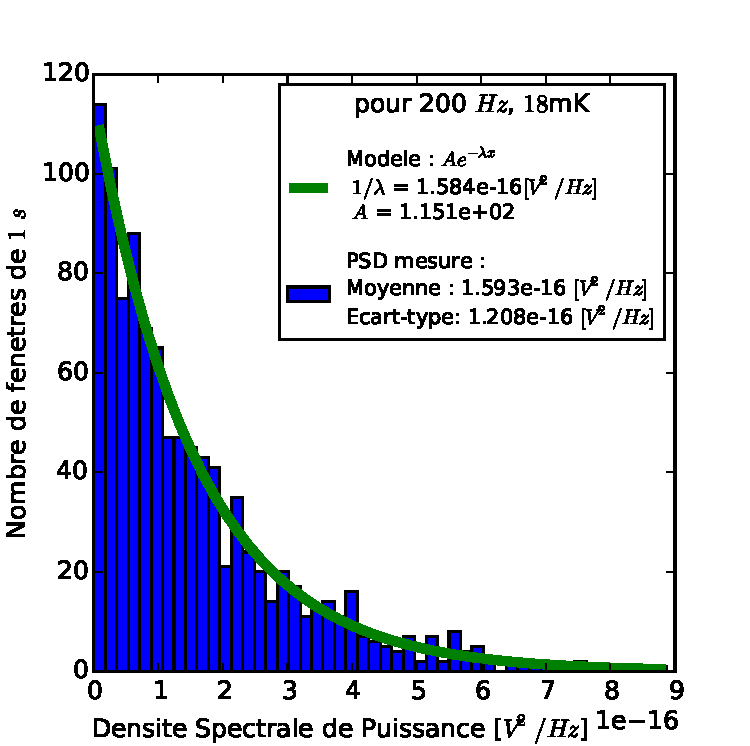
\includegraphics[width=0.6\textwidth]{Images/fit_exp_fin.pdf}
\end{center}
\caption{Histogram of the noise spectral density at $200 Hz$ adjusted by an exponential model.}
\label{noise-form}
\end{figure}

In a first step, the histogram of the measured PSD value for different frequencies is plotted. Such a histogram is presented for a frequency of $200$Hz on the figure \ref{noise-form}. Regardless of the frequency probed, the temperature of the cryostat, or the electronics used, a similar distribution pattern is observed. An exponential distribution is successfully fitted to these histograms. A property of the exponential distribution can be applied to the noise: the mean value $\mathcal{D}_i$ of a measurement at frequency $i$ is equal to its standard deviation $\sigma_{\mathcal{D}_i}$. Indeed, the experimental values of the mean and the standard deviation are close to the term $1/\lambda$.
Thus, on a measure averaged over $N=120$ windows of $1$ second, the Central Limit Theorem expresses the standard deviation on the averaged measure $\sigma_{\bar{\mathcal{D}}_i}$ such that:
\begin{equation}
\label{sigma}
\sigma_{\bar{\mathcal{D}_i}} = \frac{\sigma_{\mathcal{D}_i}}{\sqrt{N}} = \frac{\bar{\mathcal{D}_i}}{\sqrt{120}}
\end{equation}

This information on the PSD of the noise allows to rigorously construct a likelihood function based on the $\chi^2$ function related to the noise model with the parameters $\Theta$ and the experimental data $\mathcal{D}$. It is written as :
\begin{equation}
\label{chi2}
\chi ^2 (\Theta|\mathcal{D}) = \sum^{N_{Temp}}_{j} \sum^{N_{bin}}_{i} \left[ \frac{\bar{\mathcal{D}_{ij}} - \mathcal{M}(f_{ij}; \Theta)}{\sigma_{\bar{\mathcal{D}_{ij}}}} \right]^2
\end{equation}
where we sum over the set of frequencies $N_{bin}$ and over the set of measurement temperatures $N_{Temp}$. In fact, the model is simultaneously adjusted on several PSD measurements carried out for temperatures ranging from $18$mK to $40$mK. We thus hope to obtain better constraints on the parameters, firstly because more points are analyzed, but above all because the change in temperature modifies system parameters (in particular the resistance of the NTD $R(T_e)$) and removes the problems of degeneration between the different free parameters.

Motivated by a Bayesian approach \cite{julian}, the likelihood function is expressed as,
\begin{equation}
\label{likelihood}
\mathcal{L}(\Theta | \mathcal{D}) = \exp{\left(\frac{-\chi ^2 (\Theta|\mathcal{D})}{2}\right)}
\end{equation}

\subsection{Monte Carlo Markov Chain Monte Carlo Analysis (MCMC)}


We look for the set of parameter $\Theta$ that minimizes the likelihood function $\mathcal{L}(\Theta | \mathcal{D})$. To do this, we apply a Markov Chain Monte Carlo analysis called the MCMC method. It is a method based on random walk with condition of one (or more) Markov chain, a set containing the free parameters, in the dimensional space $N=7$ corresponding to the number of free parameters. It has been shown that with a correct likelihood function, the Markov chain allows to sample this function in a neighborhood of the optimal solution . The advantages of the MCMC method are that it can probe a large part of the free parameter space but that it converges quickly to the neighborhood of the optimal solution which can then be explored and analyzed with histograms of Markov chain positions. The figure (\ref{triangle-mcmc}) shows such histograms for EDELWEISS electronics.
\begin{figure}
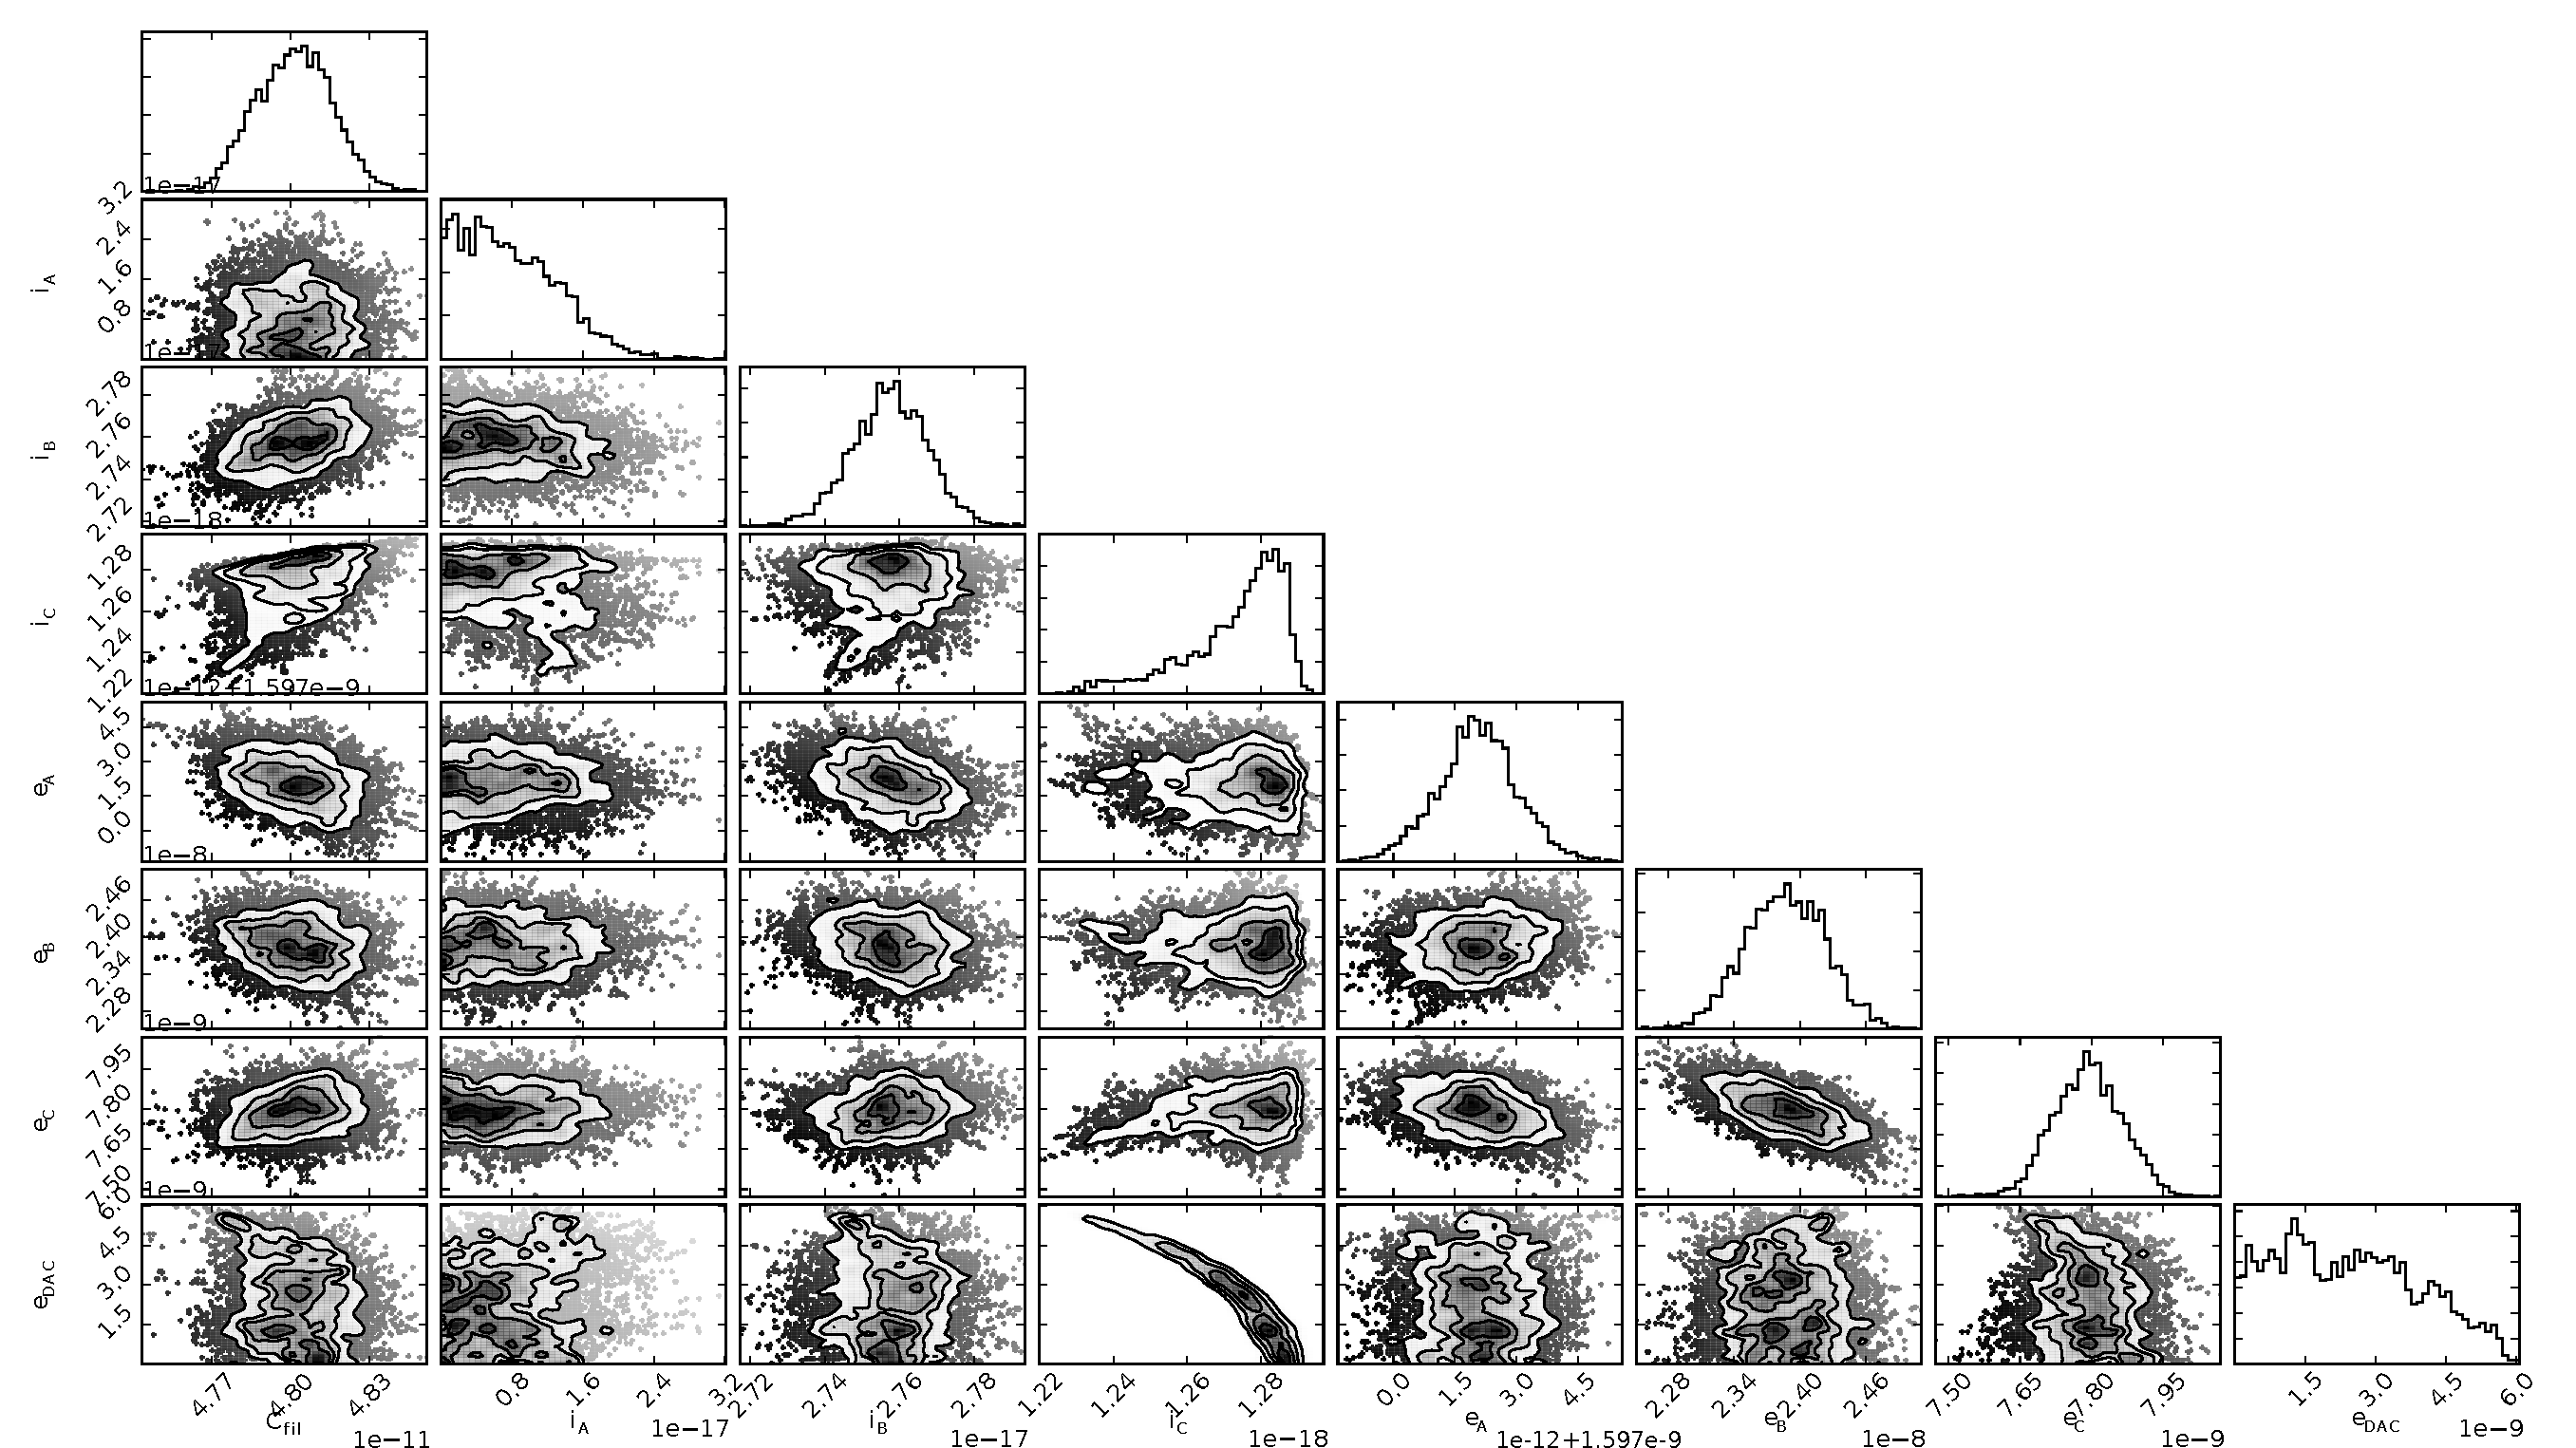
\includegraphics [width=\textwidth]{Images/triangle_fin.pdf}
\caption{Histogram of Markov chain positions with 2-dimensional projections, during MCMC analysis for EDELWEISS electronics. The free parameters presented are from top to bottom, and from left to right: $C_{thread}, i_A, i_B, i_C, e_A, e_B, e_C, e_{DAC}$.}.
\label{triangle-mcmc}
\end{figure}
From the position histogram, the mean position is extracted as an estimate of the set of optimal free parameters as well as the $68\%$ error bars on this estimate from the 16th and 84th quantiles of the distributions. The shape of the distributions also informs us about the quality of the constraint imposed on the considered parameter. Indeed, a narrow distribution indicates a well constrained parameter (parameter $i_B$) with small error bars contrary to a spread distribution which predicts large error bars (parameter $i_A$). Two parameters whose projection in 2 dimensions is elongated indicates their correlation (parameter $i_C$ and $e_{DAC}$). 

\begin{figure}[!ht]
\begin{center}
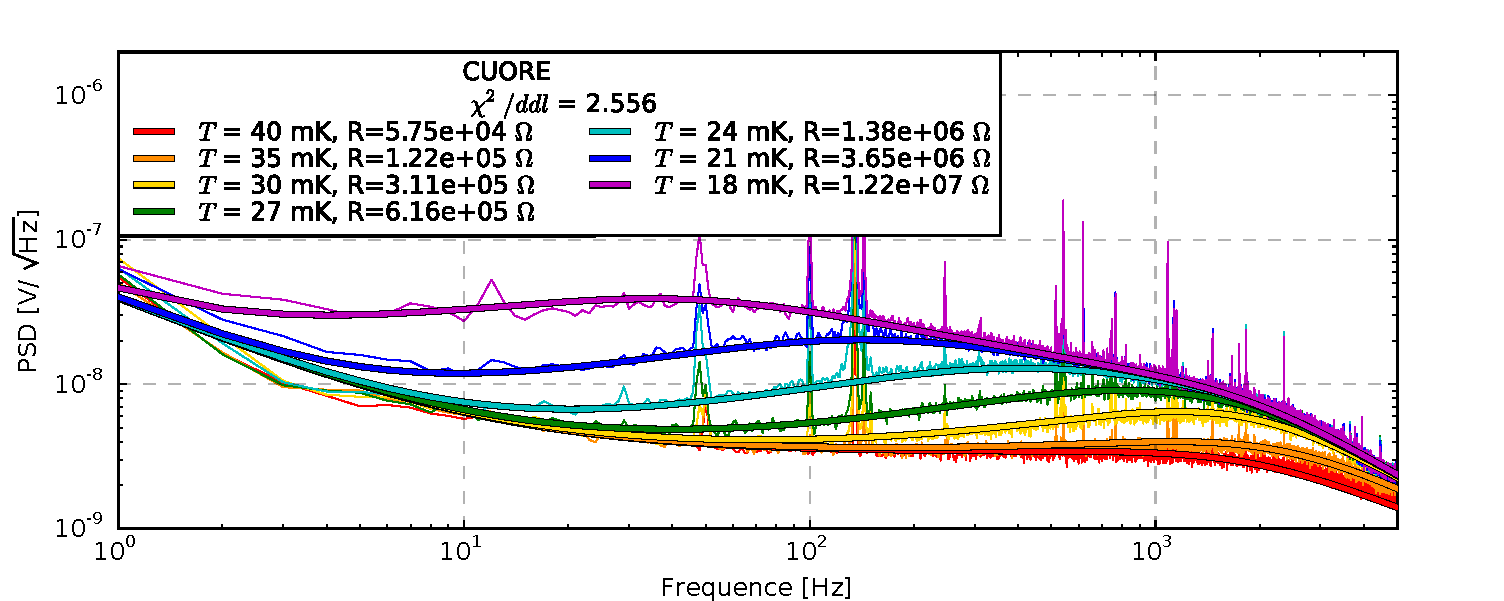
\includegraphics[width=\textwidth]{Images/cuore_fit_fin.pdf}
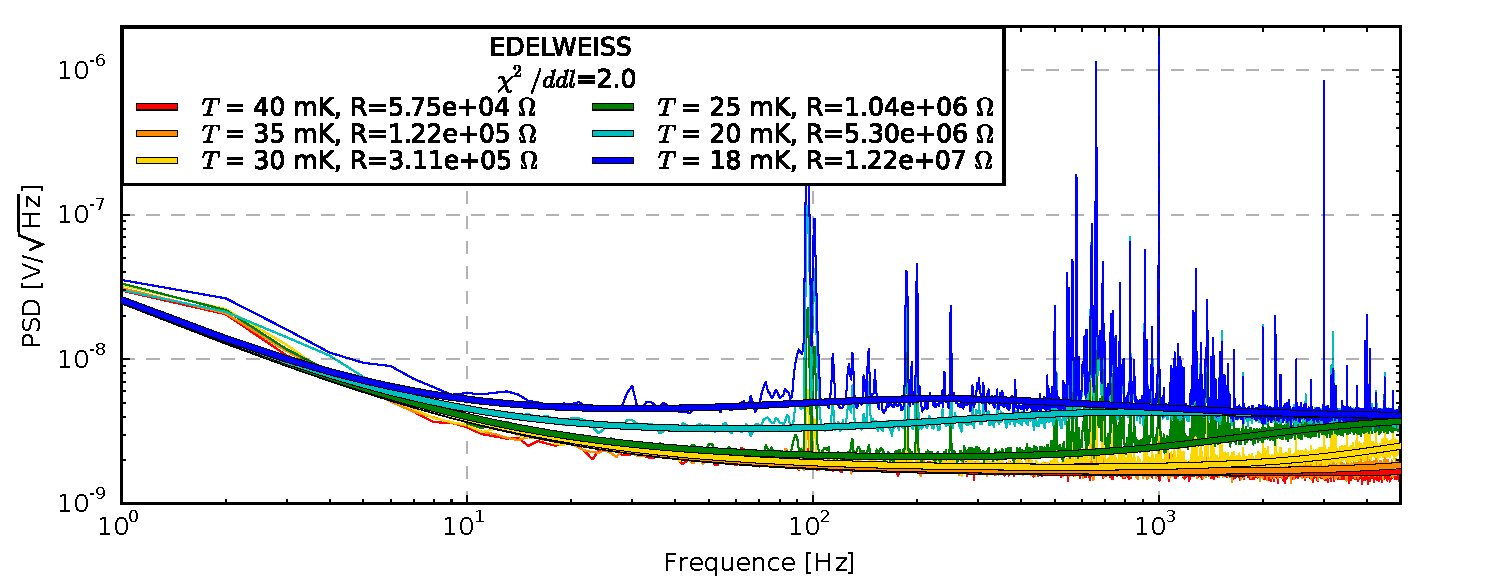
\includegraphics[width=\textwidth]{Images/edel_fit_fin.pdf}
\end{center}
\caption{Averaged measurements (thin lines) and adjustment by MCMC analysis (thick lines) of noise spectral densities for different temperatures on both electronics: CUORE and EDELWEISS. It is important to note that these are noise measurements performed without polarization current. For each cryostat temperature $T$ is specified the value of the thermistor $R$. The term $\chi^2/ddl$ indicates the value of the function $\chi^2$ divided by the number of points (degrees of freedom) of the fit. For a perfect modeling of the experimental data: $\chi^2/ddl \rightarrow 1$}
\label{rainbow-plot}
\end{figure}

After MCMC analysis, we obtain the fit of the experimental data relating to CUORE and EDELWEISS electronics presented in the figure (\ref{rainbow-plot}). The adjustment was performed on the PSD envelope, the parasitic peaks were ignored for the analysis. For the CUORE electronics, a cut-off above $2$kHz is observed: this comes from a low-pass filter integrated in the electronics. It has been taken into account and therefore does not affect the convergence of the MCMC for CUORE. We also note the appearance of two additional free parameters. The $f_B$ parameter corresponds to the order of the low-pass filter for CUORE measurements. The parameter $e_{DAC}$ corresponds to the noise of a power supply connected in series with the capacity of the EDELWEISS electronics. The addition of these additional parameters gives more flexibility to the model so that it better adapts to the experimental data, and thus does not distort the optimal solution.

\begin{align}
\label{result}
\begin{aligned}[c]
& \textrm{\textbf{CUORE}} \\
C_{fil} &= (2.94 \pm 0.01)\times 10^{-10}&[F] \\
i_A &= (1.9 \pm 0.03) \times 10^{-15}&[A/\sqrt{Hz}] \\
i_B &= (6.11 \pm 0.01) \times 10^{-16}&[A/Hz] \\
i_C &= (1.16 \pm 0.01) \times 10^{-17}&[A/Hz^{3/2}] \\
e_A &= (3.28 \pm 0.01) \times 10^{-9} &[V/\sqrt{Hz}] \\
e_B &= (3.03 \pm 0.04) \times 10^{-8}&[V] \\
e_C &= (1.08 \pm 0.02) \times 10^{-8} &[V \cdot \sqrt{Hz}] \\
f_B &= (2.70 \pm 0.01) & [u.a.]
\end{aligned}
\quad \vrule{} \quad
\begin{aligned}[c]
& \textrm{\textbf{EDELWEISS}} \\
C_{fil} &= (4.80 \pm 0.02)\times 10^{-11}&[F] \\
i_A &= (6.17 \pm 4.8) \times 10^{-18}&[A/\sqrt{Hz}] \\
i_B &= (2.76 \pm 0.01) \times 10^{-19}&[A/Hz] \\
i_C &= (1.28 \pm 0.02) \times 10^{-18}&[A/Hz^{3/2}] \\
e_A &= (1.60 \pm 0.00) \times 10^{-9} &[V/\sqrt{Hz}] \\
e_B &= (2.39 \pm 0.04) \times 10^{-8}&[V] \\
e_C &= (7.81 \pm 0.07) \times 10^{-9} &[V \cdot \sqrt{Hz}] \\
e_{DAC} &= (2.02 \pm 1.9) \times 10^{-9}&[V/\sqrt{Hz}] 
\end{aligned}
\end{align}

We check that the fit is excellent on all frequencies, with a certain reserve for the low frequencies of the CUORE electronics. Indeed, the function of $\chi^2$ weighted by the number of degrees of freedom $ddl$ is equal to $2.556$ for CUORE and $2.0$ for EDELWEISS, which is close to the $1$ value corresponding to a perfect modeling. The optimal solutions, indicated in (\ref{result}), for the electronics allow to simulate well the noise of the electronics from the proposed model (\ref{i-ampli}, \ref{e-ampli}). Different behaviors are observed depending on the temperature of the cryostat.  By noting, thanks to the equation (\ref{ode-mat}) and the \ref{block-diagram}, that the contribution of the current noise $i_{noise}$ increases with the complex impedance $Z_{eq}$, we can explain that the PSD levels are higher at low temperature. Indeed, the NTD resistance $R(T_e)$ increases very strongly when the temperature of the cryostat decreases, so the complex impedance $Z_{eq}$ also increases.

The low-frequency behavior of the two electronics is very similar: one observes a strong rise at low frequencies associated with the parameters $e_{B,C}$. At higher frequencies, we note that the electronics of CUORE are much more sensitive to temperature than EDELWEISS. For all temperatures, the noise level of the CUORE electronics is higher than that of EDELWEISS. We simply have a factor of 2 at $40$mK while we have almost an order of magnitude difference at $18$mK. The results \ref{result} show a difference of two orders of magnitude between the current noise $i_A$ of CUORE and that of EDELWEISS. The latter is coupled to the complex impedance $Z_{eq}$ and explains the measured noise level.

\begin{figure}[!ht]
\begin{minipage}{0.49\textwidth}
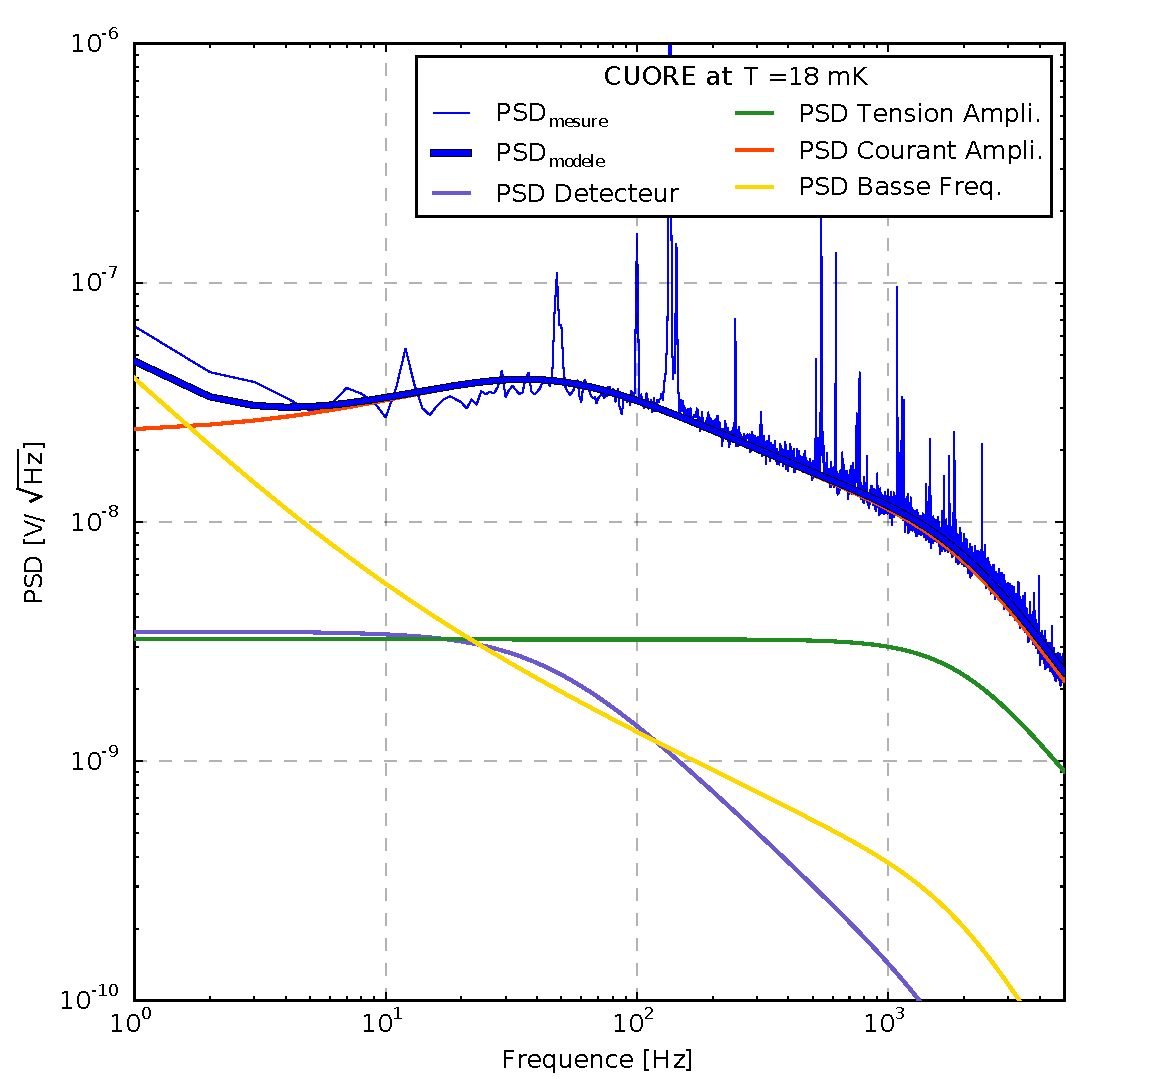
\includegraphics[width=\textwidth]{Images/cuore_18.pdf}
\end{minipage}
\hfill
\begin{minipage}{0.49\textwidth}
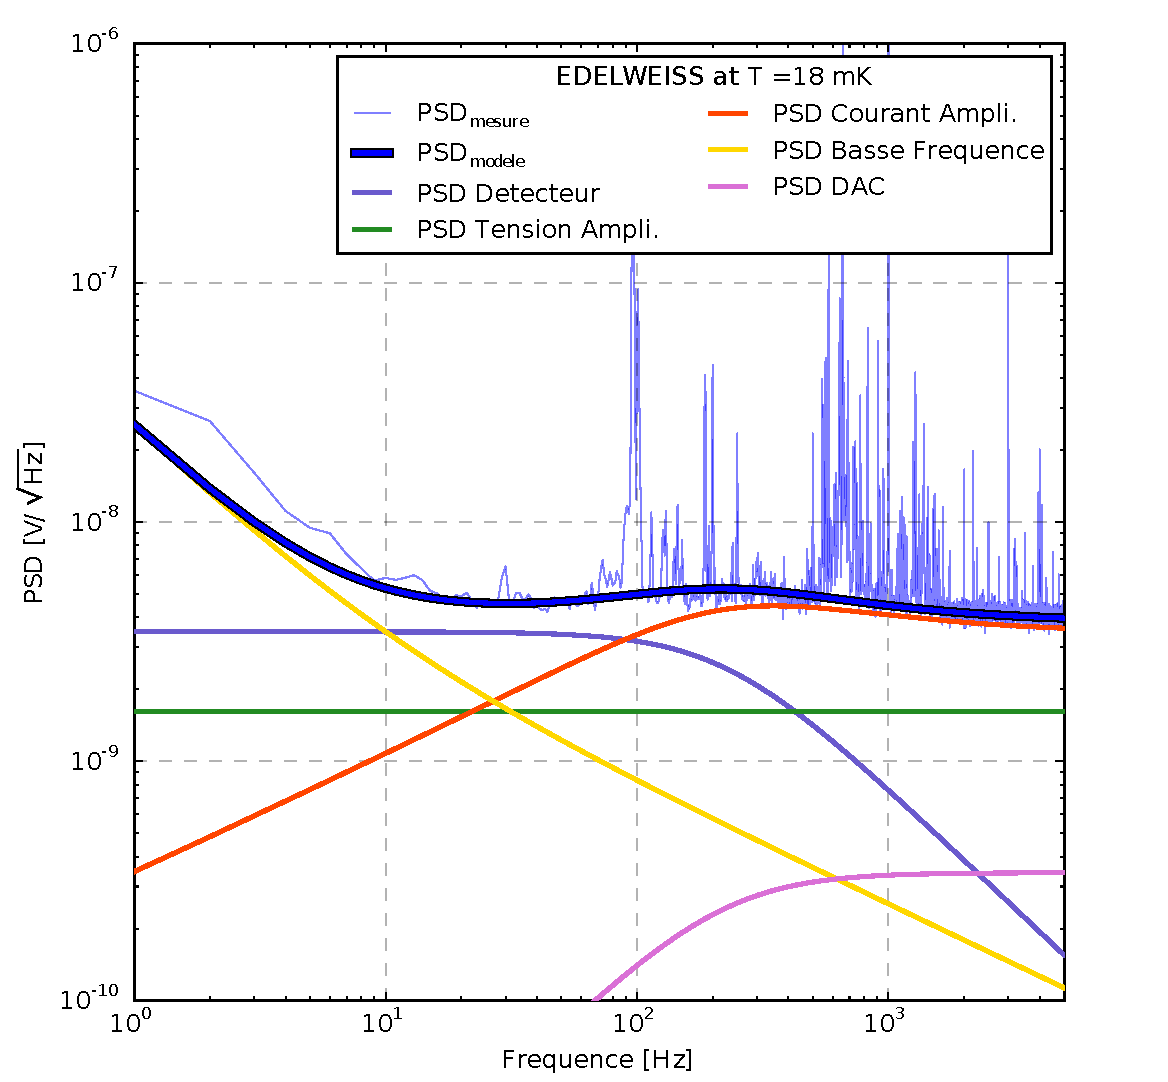
\includegraphics[width=\textwidth]{Images/edel_18.pdf}
\end{minipage}
\caption{Experimental measurement and model of a noise spectral density at $18$ mK for CUORE (left) and EDELWEISS (right) electronics with visualization of the contributions of the different noise sources.}
\label{noise-sources}
\end{figure}

It therefore appears that the least noisy electronics is that of EDELWEISS. It is thus with this electronics that it is agreed to optimize the resolution of the detectors. Nevertheless, the EDELWEISS electronics require certain modifications in order to be used with a non-zero polarization (replace the capacitance by a load resistor). This being at the project stage, only the CUORE electronics can be used for measurements with polarization to characterize the RED10 detector. As it has also been characterized, this does not pose any particular problems.

Using the optimal solution found with the MCMC analysis, it is possible to visualize the contributions of the different noise sources to the total noise PSD, an example at $18$mK is shown in figure \ref{source-noise} for the electronics of CUORE and EDELWEISS. It can be seen that the current noise of CUORE is very high and dominates almost the whole frequency range. The Johnson noise cut-off frequency, which is different for the two electronics, illustrates the influence of the wiring capacity. Indeed, we have $f_{cut} = 2\pi/(R_{NTD} C_{fil})$ considering $R_L\gg R_{NTD}$. A higher cut-off frequency is found in the case of EDELWEISS which has a lower wiring capacity (see \ref{result}). It is also possible to study the predominance of noise sources as a function of frequency. For the electronics of EDELWEISS :
\begin{itemize}
\item below $10$Hz, the noise is dominated by the low-frequency contributions of noise in voltage $e_{B,C}$.
From $10$Hz to $100$Hz, the total noise is based on the intrinsic noise of the detector (TFN noise and Johnson noise of the NTD). This is exactly what is sought: one seeks to be limited by these detector thermal noises which sets the ultimate attainable limit.
\item above $100$Hz, the current noise of the amplification electronics characterized by the coefficients $i_{A,B,C}$ becomes predominant.
\end{itemize} 

\begin{figure}[!ht]
\begin{minipage}{0.49\textwidth}
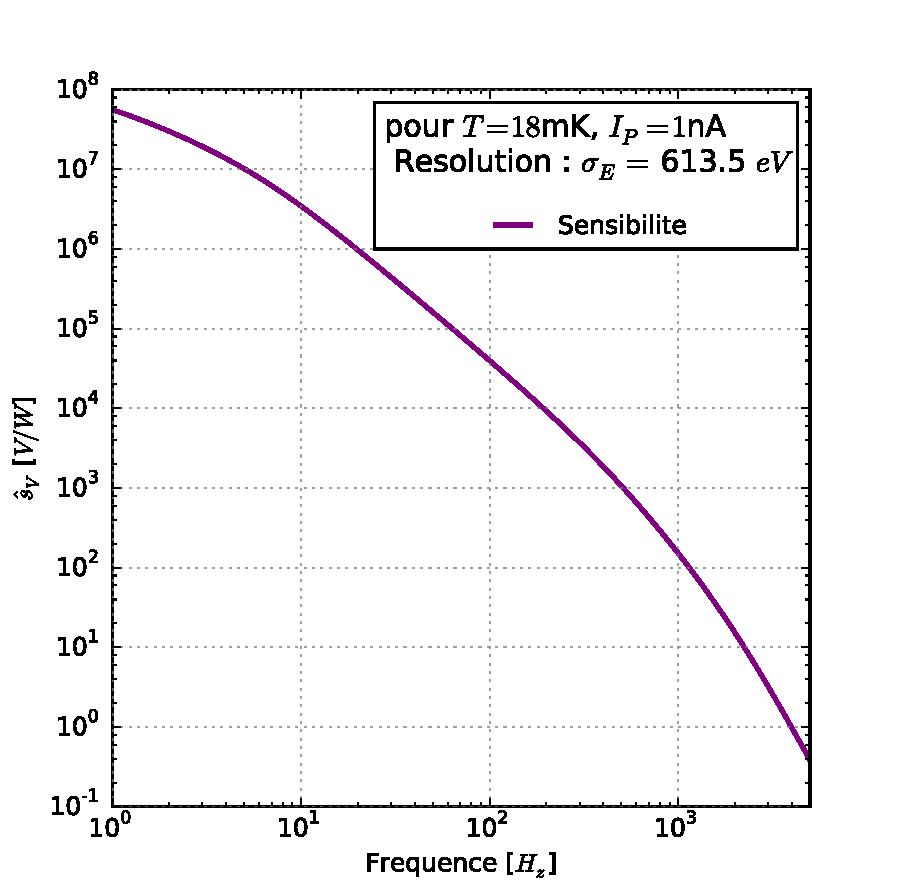
\includegraphics[width=\textwidth]{Images/sv_fin.pdf}
\end{minipage}
\hfill
\begin{minipage}{0.49\textwidth}
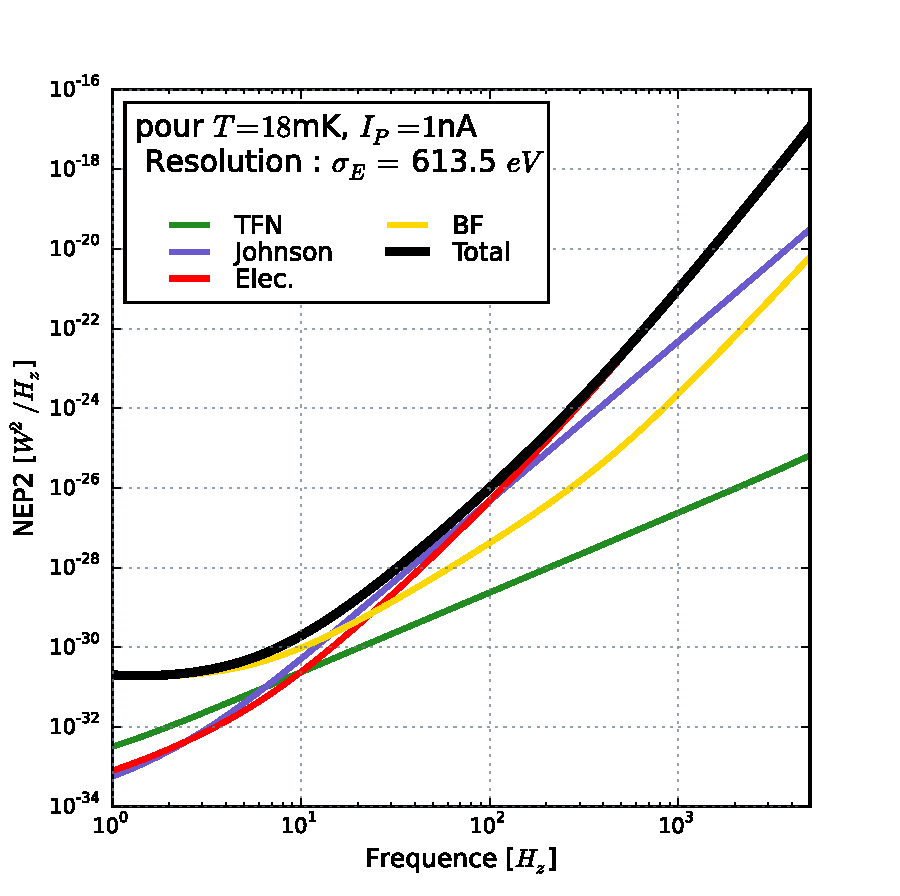
\includegraphics[width=\textwidth]{Images/nep_fin.pdf}
\end{minipage}
\caption{Simulation of sensitivity (left) and CIP (right) with contributions of different noise sources for EDELWEISS electronics at a cryostat temperature of $T=18$mK and a bias current of $1$nA.}
\label{nep-fig}
\end{figure}

\subsection{PEN plotting and resolution calculation}
\label{nep-res}

Now that we have constrained all the parameters of the noise model, it is possible to finalize the computation of the resolution \ref{resolution} with the computation of the NEP \ref{nep}. Figure \ref{nep-fig} shows sensitivity and CIP graphs of the detector with EDELWEISS electronics at $18$mK for a bias current of $1$nA. The sensitivity is consistent with the transfer function of a thermal system: it is indeed a low-pass. Combining according to the formula (\ref{nep}) this sensitivity with the PSD of total noise characterized previously allows to obtain a simulation of the CIP which presents its lowest values between $1$Hz and $100$Hz. 

%\begin{figure}[!ht]
%\begin{center}
%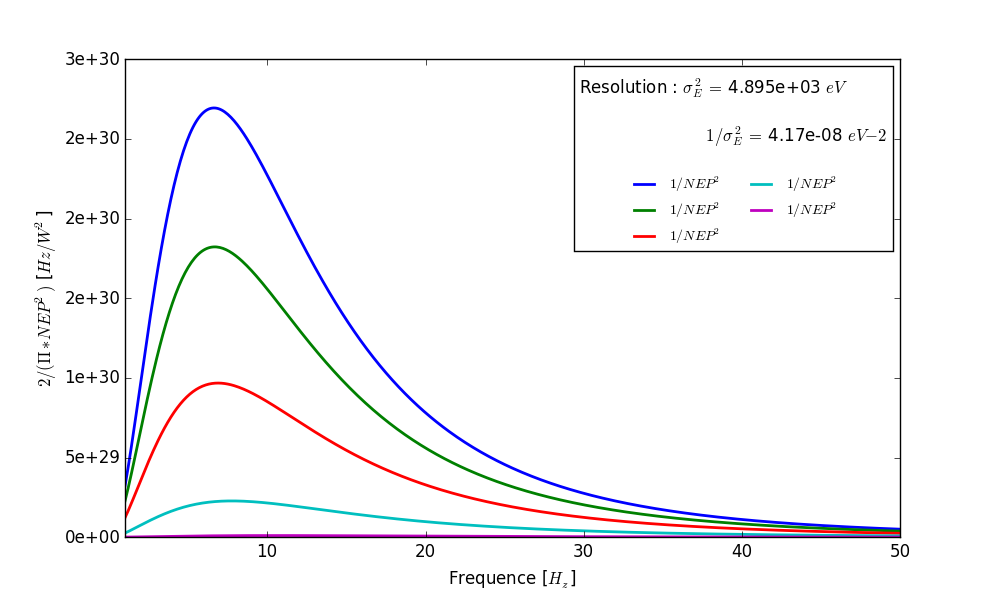
\includegraphics[width=0.7\textwidth]{Images/inte.png}
%\end{center}
%\caption{Simulation de la fonction $\frac{2}{\pi \times NEP^2(\omega)}$ qui apparaît comme intégrande dans la formule de la résolution (\ref{resolution}).}
%\label{inte}
%\end{figure}
It is now possible to access the resolution of this experiment configuration with the formula (\ref{resolution}). We calculate here a resolution of $613.15$eV for EDELWEISS, and a resolution of $1061.7$eV for CUORE, with a temperature of $18$mK and a bias current of $1$nA. A lower value is obtained with the EDELWEISS electronics, which further confirms the choice of this electronics for the optimization of the resolution.

The formula for calculating the resolution (\ref{resolution}) indicates that the lowest CIP values contribute the most to the resolution. Although integrating over a wider frequency range results in lower resolution, the gain becomes negligible as the CIP value increases.
Note that the CIP takes its minimum values around $10$Hz: most of the measurement information is contained in a frequency range from $0$Hz to about $50$Hz. The gain in resolution by integrating beyond $50$Hz is very small. The frequency range of interest for the study of the signal is then identified. By observing the contributions of the different noise sources to the CIP in figure \ref{nep-fig}, we can see that it is low frequency noise that dominates in this frequency range of interest, followed by the Johnson noise of the NTD resistor. We understand that to further decrease the resolution of these detectors, we must work to increase the sensitivity of the system to an event or reduce the low-frequency noise. Part of the Manoir team is already working to understand this low-frequency noise.

\subsection{Thermal characterization of the RED10 detector}

The RED10 detector has only recently come into the possession of the Manor group. Its design is identical to that of RED1. The difference with the latter lies in the type of glue used (glue from the CRESST experiment) and the dimensions of the NTD used. Some thermal parameters are then modified compared to RED1. It is thus necessary to characterize these thermal parameters for a new detector. One will be able to study its response to an event as it was done with RED1 in the previous parts.

\subsection{Current-voltage characteristic and signal shape}

The characterization of the thermal parameters uses the electro-thermal model that was built previously. We will want to adjust the unconstrained parameters to the experimental data with an MCMC analysis as for the characterization of the electronics. This time, the set of free parameters is :
\begin{equation}
\Theta = (R_0, T_0, g_{ep}, g_k, g_{glue}, \epsilon, \tau_P)
\label{theta-red10}
\end{equation}
Indeed, the new glue used has a different conductivity $g_{glue}$. The new geometry of the NTD (and also its slightly different neutron doping) will lead to a modification of the resistance $R_0$ and characteristic temperature $T_0$ present in the equation (\ref{ntd}). The change in dimension also impacts the electron-phonon coupling $g_{ep}$ and the Kapitza conduction coefficient $g_k$. A priori, the volumetric thermal capacities of the absorber and the NTD remain unchanged, which makes it possible to recalculate the new thermal capacities from the known dimensions of the NTD. It would have been possible to include these in the free parameters, but the choice to fix them was favored in order to avoid degeneration problems and thus better constrain the parameters.
A preliminary study of the signal shape (shown on the right of figure \ref{v2i-red10}) of RED10 revealed that the pulse decay has two characteristic time constants. This type of signal has never been observed on signal measurements performed with RED1: there is only one characteristic decay time explained by the thermal leakage to the cryostat from the electron bath with a recoil energy deposit in the absorber. The presence of a second characteristic time for RED10 can only be explained by the presence of athermic phonons as introduced in section \ref{omega}. These are phonons that do not immediately relax in the absorber, but pass through the NTD sensor before relaxing. They thus create a temperature rise directly within the NTD. The source term $\bm{F}$ in the equation (\ref{ode-mat}) is then rewritten:
\begin{equation}
\bm{F}(t-t_0) = 
\left( \begin{array}{c}
(1-\epsilon)E/C_a \
0 \\
\epsilon E/C_e \\\
0
\end{array} \right) \delta (t-t0)
\end{equation}
with $\epsilon$ the fraction of recoil energy converted into athermic phonons. The normalization constants of the general time solution (\ref{eigein-solc-expr}) depend on the source term $\bm{F}$ according to (\ref{normal}) and therefore differ from the case of RED1 without athermal phonons. This has the effect of better expressing a new exponential, and thus a new characteristic time, contained in the general solution. This observation of two characteristic times for the signal motivates the addition of the fraction of athermic phonons $\epsilon$ and their characteristic relaxation time $\tau_P$ to the free parameters of the model.

The current-voltage characteristics and the shape of the signal at an event of the natural radioactivity with a fixed bias current $I_P=4$nA are measured on RED10 for different temperatures ranging from $18$mK to $30$mK. Thus, we study the behavior of RED10 in the steady state (section \ref{steady-section}) and in the time regime (section \ref{temporal}).
The likelihood function analysis is performed with the MCMC method as in section \ref{caract}. Experimental data with the fitted models are presented in the figure (\ref{v2i-red10}).

\begin{figure}[!ht]
\begin{minipage}{0.49\textwidth}
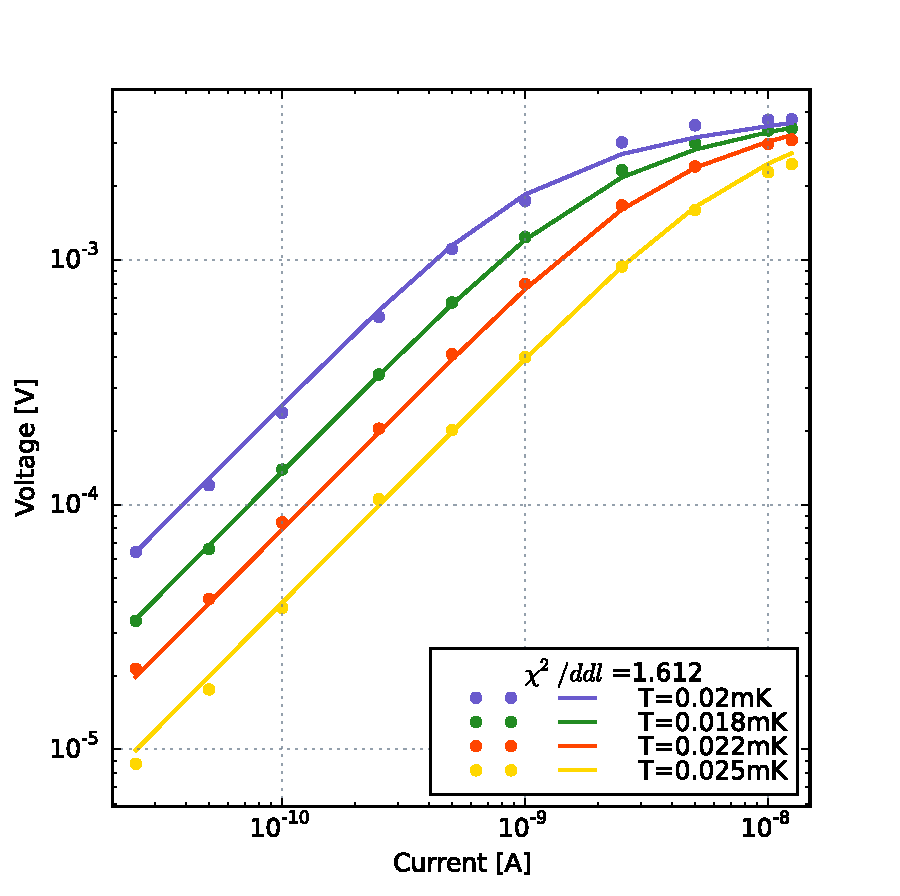
\includegraphics[width=\textwidth]{Images/v2i_red10.pdf}
\end{minipage}
\hfill
\begin{minipage}{0.49\textwidth}
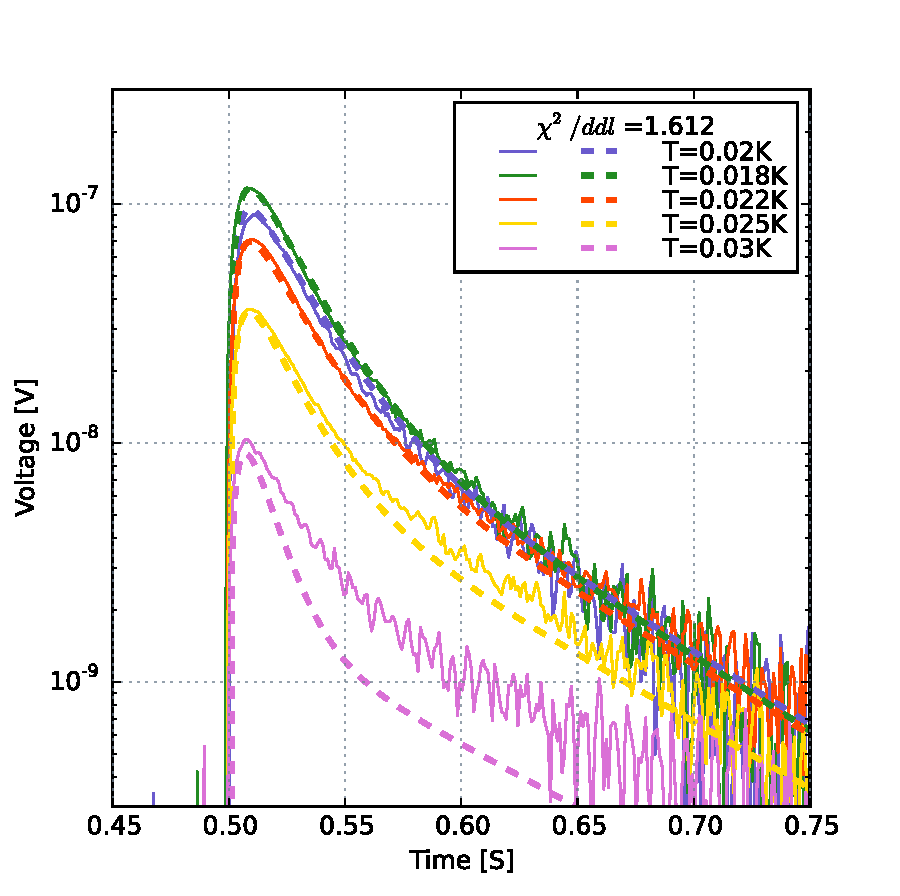
\includegraphics[width=\textwidth]{Images/pulse_red10.pdf}
\end{minipage}
\caption{Experimental measurement and model fitting of the current-voltage characteristic (left) and a signal created by an ambient radioactivity event (right) for the RED10 detector.}
\label{v2i-red10}
\end{figure}

The fit seems good for both types of measurement with $\chi^2/ddl=1,612$. However, there is a difficulty in adjusting the pulse for a temperature of $30$mK. The current-voltage characteristic makes it possible to constrain the free parameters involved in the steady state equations: $R_0, T_0, g_{ep}, g_k$. The analysis of these equations (\ref{steady}) gives us that the linear part of the characteristic constrains mainly the resistance value of the NTD, and thus $R_0, T_0$. The voltage plateau at higher bias current comes from an excessive Joule effect which is then no longer compensated by the thermal leakage to the cryostat. The NTD then increases in temperature, losing electrical resistance with a constant bias current, which causes the voltage plateau to appear. Its adjustment thus constrains the values of conductivity $g_k$ and electron-phonon coupling $g_{ep}$.

As for the shape of the signal, the model shows two slopes and thus two characteristic times. The adjustment of these two decay slopes constrains the athermic phonon fraction $\epsilon$, and more generally, all the parameters involved in the calculation of the normalization constants of the eigen-base of the solutions (\ref{eigen-soluc}).
The rise in tension allows to constrain the relaxation time of the phonons $\tau_P$. Indeed, for an immediate relaxation of the phonons, the rise time would be infinitely large (modulo the cutoff frequency $(RC_{fil})^{-1]}$).

The MCMC method then gives the following constraints for RED10:

\begin{align}
R_0 &= (11.6 \pm 0.4)&[\Omega] \\
T_0 &= (2.72 \pm 0.01) &[K] \\
g_{ep} &= (21.1 \pm 4.4) &[W/K^6/cm^3] \\
g_k &= (2.77 \pm 0.1) \times 10^{-4}&[W/K^4/mm^2] \\
g_{glue} &= (7.46 \pm 1.67) \times 10^{-4} &[W/K^{n_g}/mm^2] \\
\epsilon &= (0.202 \pm 0.001)  & [fraction]\\
\tau_P &= (4.03 \pm 0.03) \times 10^{-3} &[s]
\end{align}


These thermal parameter values are of the same order of magnitude as those corresponding to RED1. It is important to highlight the high portion of athermal phonons of about $20\%$ which is to be compared to their complete absence with the RED1 detector. This is a new observation for this type of detector. Their high presence results in an acceleration of the voltage signal and thus an increase of the frequency range of interest of the signal introduced in the section \ref{nep-res}. In addition, athermic phonons are not affected by the capacity of the absorber, and transmit all their energy directly to the NTD. Understanding and increasing the rate of athermal phonons will thus allow the resolution of the detector to be lowered. A new way of optimizing the detectors has been discovered, which is not yet considered within the EDELWEISS collaboration.

\subsection{Red10 noise and resolution}

Since RED10 is fully characterized from the thermal point of view, and the CUORE electronics used for the measurements are also characterized, we are able to simulate the noise spectrum related to RED10 compared to the experimental measurement. Figure (\ref{noise-red10}) shows the modeling and experimental measurement of the PSD of RED10 noise at a bias current of $4$nA for a temperature of $22$mK. Note that a Bessel filter is applied to the measurement, and to the model, which explains the cutoff appearing from $2$kHz.

\begin{figure}[!ht]
\begin{center}
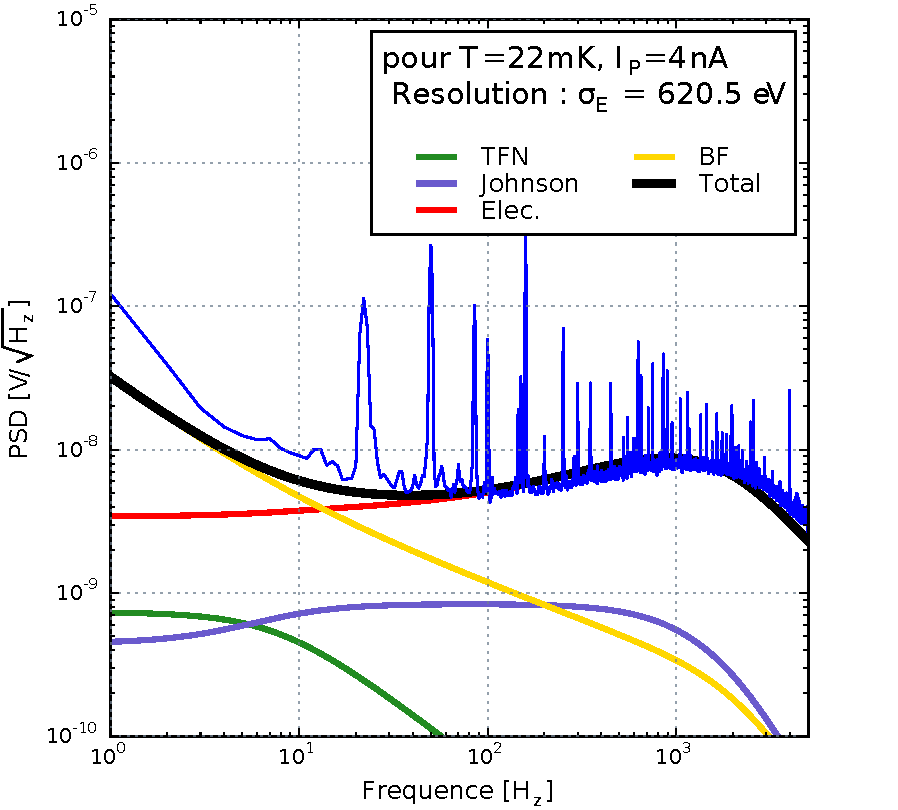
\includegraphics[width=0.55\textwidth]{Images/modexp.pdf}
\end{center}
\caption{Experimental measurement of a spectral density at $22 mK$ with RED10 compared to a simulation of the built model.}
\label{noise-red10}
\end{figure}

The model and the measurement describe very similar developments. We do find the presence of high low frequency noise that dominates up to $15$Hz. It is then the current noise that predominates over the rest of the frequency range. It should be noted that a measurement of noise with bias current is performed here, so it would be incorrect to compare the presented current noise of RED10 with the current noise of RED1 obtained without bias current. However, there is a slight shift in the model from the experimental data to the low frequencies. This can be explained by the underestimation of the low-frequency noise already observed for CUORE electronics in the figure (\ref{rainbow-plot}). The excess of low-frequency noise also comes from the high rate of muon events during the measurements: despite the cuts made in the analysis, part of the signal decay is always recovered, which helps to amplify the low frequencies of the measured spectrum.

The experimental resolution measurement is carried out from the noise PSD and the measurement of a signal. Indeed, renormalizing the amplitude of the signal and applying a Welch method allows to estimate the signal sensitivity of the RED10 detector. The renormalization also requires to know the conversion between the energy deposited in the absorber by an event and the amplitude of the measured signal. This calibration is performed using the interaction of cosmic muons with the absorber. The energy they deposit in the absorber is equal to $18$MeV. Measuring the voltage amplitude of a muon signal therefore allows to deduce the conversion factor necessary for the renormalization of a signal. The application of the discrete analogue of the formula (\ref{resolution}) to a noise spectrum and the previously calculated sensitivity allows the evaluation of an experimental resolution. 

\begin{figure}[!ht]
\begin{center}
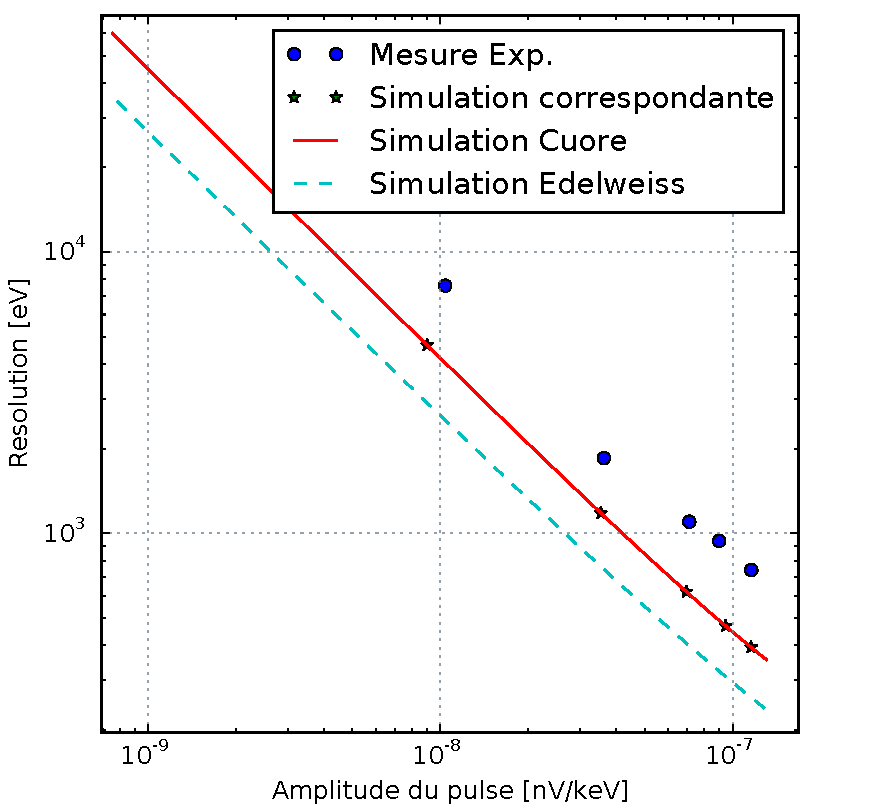
\includegraphics[width=0.55\textwidth]{Images/resamp_fin_fin.pdf}
\end{center}
\caption{Resolution-Signal amplitude characteristic for the RED10 detector for a bias current of $4$nA with temperatures ranging from $18$mK to $30$mK.}
\label{amp-res-red10}
\end{figure}


The figure (\ref{amp-res-red10}) shows the resolutions as a function of the signal amplitude for different temperatures at a fixed bias current. The experimental resolutions are higher than the simulated resolutions. This is explained by the deviation between model and noise measurement observed in figure (\ref{noise-red10}): the modeled low-frequency noise is lower than in reality, hence the prediction of lower resolutions. The pulse amplitude is used to estimate the sensitivity of RED10 to the signal. Except for the $30$mK measurement where the signal was already poorly modeled, the simulated and real amplitude values are almost identical. Moreover, since the two sets of dots show a very similar evolution of the resolution as a function of amplitude, it is deduced that the model is in good adequacy with the experimental reality. A study of the noise difference is still necessary to obtain a complete adequacy of model and experiment.

It should be noted that the measurements were performed with CUORE electronics. The simulation of the resolution-amplitude characteristic is plotted for both CUORE and EDELWEISS electronics. It should be noted that the latter makes it possible to gain almost a factor of 2 on the value of the resolution (the amplitude remains unchanged). This is consistent with the low noise level of EDELWEISS compared to that of CUORE.

\subsection{Optimization of the RED10 detector and perspectives}

An electro-thermal model was built and tested with RED10. Even if some parameters need to be further refined to have a better fit, we can perform a preliminary optimization of the RED10 detector. A simulation of the resolution of RED10 as a function of the bias current flowing through its NTD for different cryostat temperatures is presented in figure \ref{optim}. The simulation is performed with the EDELWEISS electronics which has the lowest noise level, and the temperature of the load resistor is lowered to the temperature of the mixing chamber to reduce its Johnson noise (which will be realized in the next few months).

It is observed that there is an optimum current corresponding to each temperature to minimize the resolution. Indeed, if the NTD thermistor is polarized too much, the heat produced by Joule effect can no longer be evacuated efficiently by the thermal leakage. The temperature of the NTD becomes high and therefore its value drops, which affects the sensitivity of the system. The same effect is observed when plotting the current-voltage characteristic in figure \ref{v2i-red10}. At too low a current, the NTD sensor is no longer polarized enough to efficiently convert the heat signal into a voltage signal: the sensitivity drops as well. No matter what bias current is used, the lowest resolution is always obtained at the lowest temperature. The NTD's resistance formula (\ref{ntd}) explains why the signal is more sensitive at low temperatures: the derivative of the resistance with respect to the temperature takes its maximum values there (in absolute terms). Moreover, lowering the temperature reduces all TFN noise, and the Johnson noise of the NTD thermistor, which further improves the resolution.

\begin{figure}[!ht]
\begin{minipage}{0.49\textwidth}
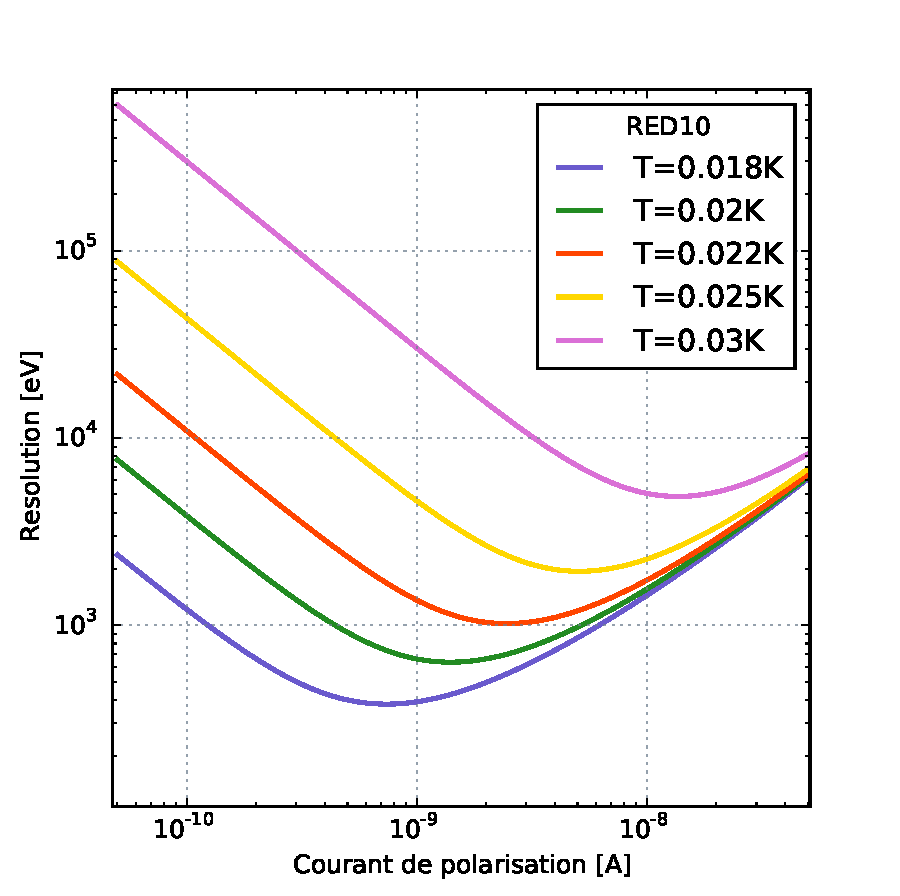
\includegraphics[width=\textwidth]{Images/red10_i.pdf}
\end{minipage}
\hfill
\begin{minipage}{0.49\textwidth}
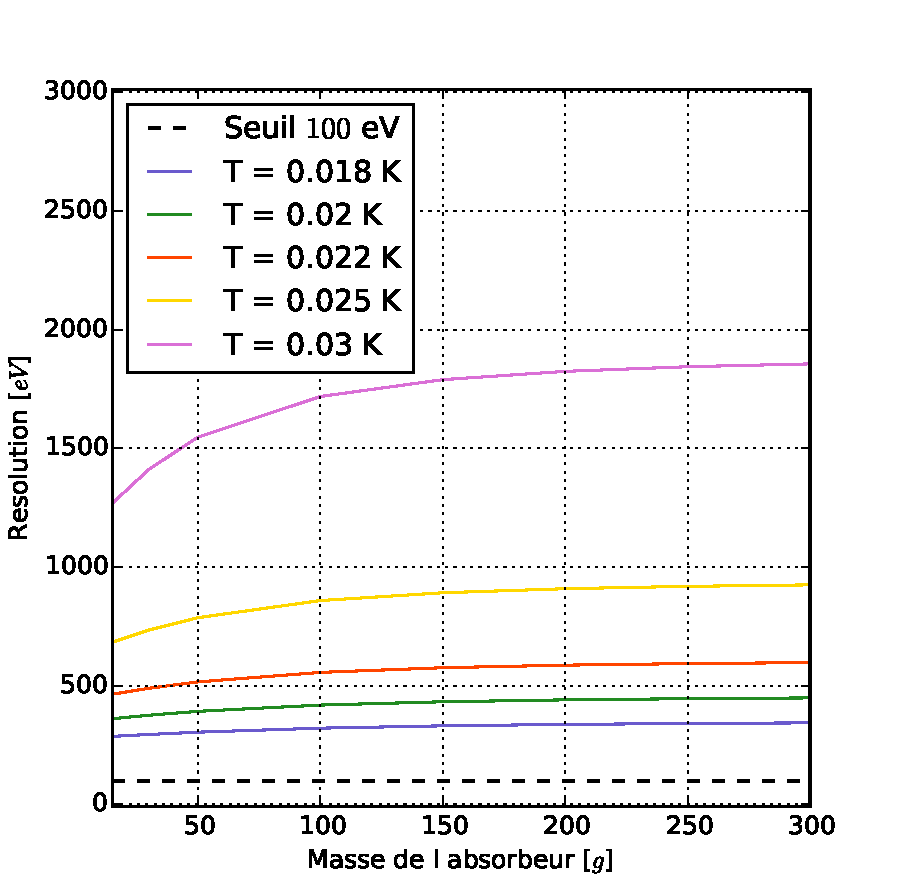
\includegraphics[width=\textwidth]{Images/red10_mass.pdf}
\end{minipage}
\caption{(left) Simulation of the resolution of RED10 as a function of the bias current for different temperatures. \\ (right) Simulation of the resolution with optimized bias current as a function of the absorber mass for different temperatures. The design considered is the same as that of RED10, only the mass of the absorber is changed by adjusting the bias current to obtain the lowest resolution.}
\label{optim}
\end{figure}

The RED10 study was fully realized for a bias current of $4$nA, which corresponds to the optimal current at a temperature of about $24$mK. It would therefore have been possible to obtain better resolution values by adjusting the bias current for each temperature. Thus, it will be important, in the future, to properly determine the optimum polarization current of a detector according to the measurement conditions.

The search for light dark matter requires the development of a new generation of detector with very low detection threshold. For this, it is necessary to work on the design of the detectors. For example, it is necessary to study the behavior of the detector according to the geometry of the NTD, the mass of the absorber or the location of thermal leaks. A simulation of the resolution of a detector as a function of the absorber mass is shown in the graph on the right side of figure \ref{optim}. Note that the polarization current is adjusted for each point to draw an already optimized resolution curve. According to the formula (\ref{capa}), it would be interesting to reduce the thermal capacity of the absorber $C$, by lowering its mass, in order to cause a greater temperature rise $\Delta T$, and thus amplify the heat signal. According to the simulation, this amplification of the heat signal would appear only for very small detector masses, and would remain very modest for low temperatures. 

It is now understood that we remain limited for the moment by another aspect of the detector. In the future, the optimization of the detector will involve the study of the behavior as a function of the dimensions of the NTD thermistor and the thermal conduction surfaces. It already appears that it would be necessary to reduce the thermal capacities of the different baths while maximizing the thermal bonds. 

